% \documentclass[a4paper,10pt,unnumberedsections,twoside]{LTJournalArticle}
% \documentclass{IEEEtran}
\documentclass[12pt]{assignment}
% \documentclass{article}

\usepackage{float}
\usepackage{hyperref}
\usepackage{graphicx}
\usepackage{xcolor}
\usepackage[export]{adjustbox}
\usepackage{enumitem}
\usepackage{tikz}
\usepackage{braket}


\hypersetup{
pdftitle={ME738 - Special Topics in Materials},
pdfsubject={Project report},
pdfauthor={Tommaso Bocchietti}
}

\makeglossaries
\newacronym{csac}{CSAC}{Chip-Scale Atomic Clock}
\newacronym{csacs}{CSACs}{Chip-Scale Atomic Clocks}
\newacronym{pp}{PP}{Physics Package}
\newacronym{cl}{CL}{Control Loop}
\newacronym{lo}{LO}{Local Oscillator}
\newacronym{fs}{FS}{Frequency Synthesizer}
\newacronym{modr}{MODR}{Microwave Optical Double-Resonance}
\newacronym{cpt}{CPT}{Coherent Population Trapping}
\newacronym{rb}{Rb}{Rubidium}
\newacronym{cs}{Cs}{Cesium}

% \addbibresource{references.bib}

% \runninghead{Chip Scale Atomic Clocks}

% \footertext{ME738 - Special Topics in Materials}

% \setcounter{page}{1}

\title{Chip Scale Atomic Clocks: current status and future prospects}
\author{Tommaso Bocchietti}
\date{\today}

% \author{
% 	Tommaso Bocchietti\textsuperscript{1,2}\thanks{\textbf{Final revision:} April ??, 2024}
% }

% \date{\footnotesize{
% 	\textsuperscript{\textbf{1}}Department of Mechanical \& Mechatronics Engineering, University of Waterloo\\
% 	\textsuperscript{\textbf{2}}Dipartimento di Meccanica, Politecnico di Milano
% 	}
% }

% \renewcommand{\maketitlehookd}{}

\begin{document}

% \maketitle

% \begin{figure}[H]
% 	\centering
% 	
\includegraphics[width=.9\textwidth]{./pdf/UniversityOfWaterloo_logo_vert_pms}
% 	\label{fig:University_Of_Waterloo_logo}
% \end{figure}

% \clearpage
% \section*{Abstract}

\acrfull{csacs} can be considered as one of the most significant advancements in timekeeping technology considering their low power consumption, small size, and high stability and accuracy in frequency.
Originally developed for military purposes, \acrshort{csacs} have found applications in various fields where accurate timekeeping and portability are essentials, such as satellite navigation, oil industry exploration, telecommunications, and space experimental physics.

This report will provide an overview of the key parameters, discuss the governing physics highlighting the bottleneck and limitations, and explore their current and potential applications across different sectors.
A final section will focus on the future prospects and challenges in the development of the \acrfull{ngcsacs} technology.

\vspace{1cm}

\begin{figure}[H]
    \centering
    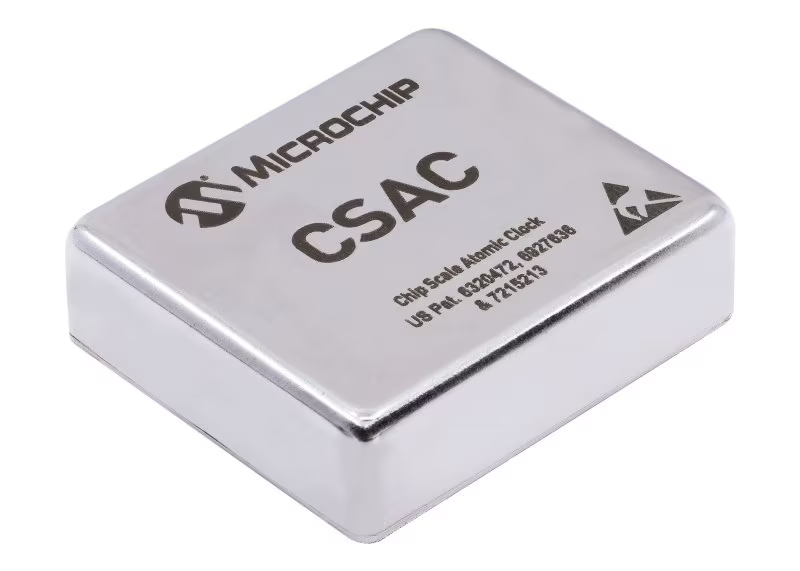
\includegraphics[width=.6\textwidth, max width=.8\linewidth]{img/microsemi-SA65.png}
    \caption{
        Microsemi SA.65 represents, since 2021, the most advanced commercially available \acrshort{csac}.
        Source: \cite{MICROCHIP}.
    }
    \label{fig:microsemi_SA65}
\end{figure}

% \clearpage
% \tableofcontents
% % \listoffigures
% % \listoftables

% \clearpage
% \section{Introduction}

Every electronic device requires the use of a timing system (usually referred as clock) that sets the reference for the operation of the device.
This timing system is implemented through the use of various electronic components such as clock source, phase comparator, frequency dividers, \dots.

The aim of this project is to investigate the state of the art of clock sources technologies, with a focus on the most recent advancements in the field and their potential applications.
In particular, the project will focus on the following topics:

\begin{itemize}
    \item \semph{Crystal oscillators}: electric oscillator type circuit that uses a piezoelectric resonator, a crystal, as its frequency-determining element (\href{https://en.wikipedia.org/wiki/Crystal_oscillator#Terminology}{Wikipedia definition}).
    \item \semph{\acrshort{mems} resonators}: small electromechanical structures that vibrate at high frequencies (\href{https://en.wikipedia.org/wiki/Microelectromechanical_system_oscillator#Resonators}{Wikipedia definition}).
    \item \semph{\acrshort{mems} Atomic Clocks} (time permitting): the combination of a \acrshort{mems} system fabrication with atomic clocks for small, cheap, low-power devices \cite{KNAPPE2008571}.
\end{itemize}



% \section{Objective metrics for timekeeping devices}
\label{sec:objective_metrics}

Before diving into the core subject of \acrfull{csacs}, it's important to give some definitions and explain the key parameters that define the performance of these devices.
Those parameters will be used in section \ref{sec:working_principles} as objective metrics to compare and highlight the major differences between various types of \acrshort{csacs} and other types of clocks.

\subsection{Second ([s]) definition}
\label{subsec:second_definition}

The Bureau International des Poids et Mesures (BIPM), which is one of the three organizations that define the International System of Units (SI), defines the second as: \textit{the fixed numerical value of the $Cs$ frequency $\Delta \nu_{Cs}$, the unperturbed ground-state hyperfine transition frequency of the $^{133}Cs$ atom, to be $9.192.631.770$ when expressed in the unit $Hz$, which is equal to $s^{-1}$.}

This kind of definition was first adopted starting from the year 1967, when experimental work showed the accuracy and reproducibility of transition between two energy levels of an atom or a molecule.
The current definition of the second was proposed and adopted starting from 2018, and it's also at the basis of the modern atomic clocks.


\subsection{Stability}
\label{subsec:stability}

Stability, when referring to a clock source, is the measure of how well the reference frequency can be maintained over time.
All the metrics used to define the stability of a clock are based on the fractional frequency error, which is the ratio between the frequency error and the reference frequency, namely:

\begin{equation}
  y(t) = \frac{f(t) - f_0}{f_0}
  \label{eq:fractional_frequency_error}
\end{equation}

Where $f(t)$ is the frequency of the clock at time $t$, and $f_0$ is the nominal frequency of the clock.

In the framework of \acrshort{csacs}, or more in general of atomic clocks, three main regions can be identified in the stability plot: short-term, medium-term, and long-term stability.

\begin{figure}[H]
  \centering
  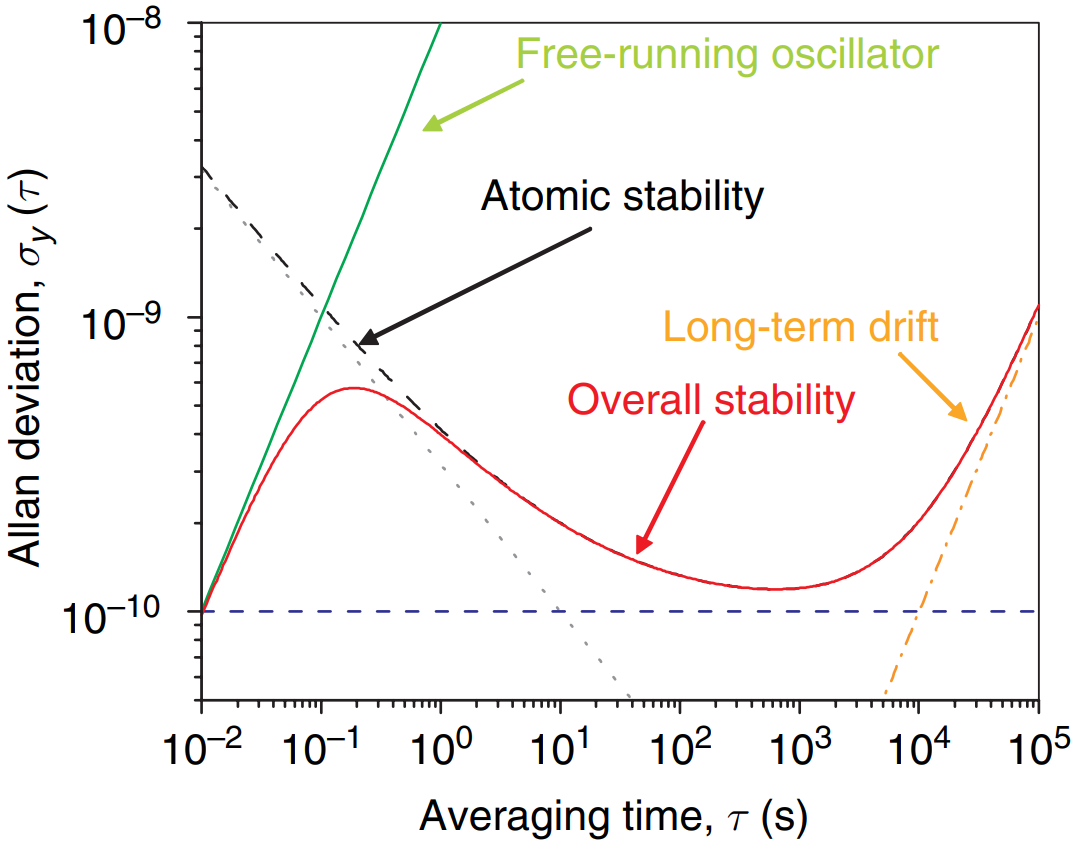
\includegraphics[width=0.6\textwidth, max width=\linewidth]{img/overall-statbility-contributions.png}
  \caption{
    Overall stability of a clock source as summation of the different contributions from the internal components and processes.
    Observing the overall stability (red line), we can distinguish three main regions: short-term ($0 \le \tau \le 10^{0}s$), medium-term ($10^0 \le \tau \le 10^{3}s$), and long-term (beyond the flicker floor).
    Source \cite{Knappe}.
  }
  \label{fig:overall-statbility-contributions}
\end{figure}

\subsubsection{Short-term stability}

Short-term stability refers to the performance of a clock over very short time intervals, typically ranging from a few milliseconds to a few seconds.
Allan deviation (denoted as $\sigma_y(\tau)$) is the metric used to measure it, capturing both rapid fluctuations (Fast Noise) and gradual drifts (Slow Drift) in the output frequency.
From its definition, Allan deviation (ADEV) can be computed as:

\begin{equation}
  \sigma_y(\tau) = \sqrt{\frac{1}{2M} \sum_{i=2}^{M} (\bar{y}(\tau)_{i} - \bar{y}(\tau)_{i-1})^2}
  \label{eq:allan_deviation_short}
\end{equation}

Where $\bar{y}(\tau)_{i}$ is the average fractional frequency error over the time interval $\tau$ and $M$ is the number of sampling data.

To give a more practical example, we can consider a clock running with an output frequency of $f_0 = 10MHz$, having an Allan deviation of $\sigma_y(\tau=1s) = 3 \times 10^{-9}$.
In this case, the instability in frequency between two observations 1 second apart has an RMS value of $3 \times 10^{-9}$, that means a $10MHz * 3 \times 10^{-9} = 30mHz$ RMS\footnote{RMS: Room Mean Square} movement in frequency mostly due to the Fast Noise.

As we will see in Section \ref{sec:performances_and_limitations}, for a \acrshort{csac} clock the component having a major impact on the Fast Noise is the \acrfull{lo}.


\subsubsection{Medium-term stability}

Medium-term stability refers to the performance of a clock over longer time intervals, typically ranging from a few seconds to a few minutes or hours.
Allan deviation is again the metric used to measure it.
In this case however, ADEV can be computed using an approximated version of Equation \ref{eq:allan_deviation_short}:

\begin{equation}
  \sigma_y(\tau) = \frac{1}{Q \times SNR} \tau^{-1/2}
  \label{eq:allan_deviation_medium}
\end{equation}

Where $Q = \frac{\nu_0}{\Delta \nu}$ and $SNR = \frac{P_{signal}}{P_{noise}}$ are related to the quality of the output signal in terms of frequency and power.

This simplified version of the Allan deviation can be adopted knowing that Fast Noise is no longer the main source of instability, and the Slow Drift becomes the dominant factor.

As we will see in Section \ref{sec:performances_and_limitations}, for a \acrshort{csacs} clock, the cause of the medium-term stability cannot be brought back to a single component, but it's the result of multiple and concurrent effects.

\subsubsection{Long-term stability}

Long-term stability refers to the performance of a clock over very long time intervals, typically ranging from a few days to a few years.
Fractional frequency error is the metric used to measure this, and it's computed from the definition given in Equation \ref{eq:fractional_frequency_error}.

It's common to consider as the starting point from which consider long-term stability region, the flicker floor.
On a $\sigma_y(\tau)$ plot, the flicker floor can be identified as the point where the Allan deviation reaches a minimum value and then starts to increase again.

At such long time scale, multiple factors influence this metric as for example aging, environmental conditions, and other external factors.
The summation of all these factors is usually referred to as Drift.


\subsection{Other metrics}
\label{subsec:other_metrics}

While stability is probably the most important parameter to define the performance of a clock, other metrics are also used to give a more complete overview of the device.
Some of the most important ones are:

\begin{itemize}
  \item Phase noise $\mathcal{L}(f)$: represents the noise power relative to the carrier contained in a 1 Hz bandwidth centered at a certain offset from the carrier. It's typically expressed in units of $dBc/Hz$.
  \item Temperature sensitivity $tempco$: measures how much the clock's performance varies with temperature changes. It's typically expressed in units of $ppb/^\circ C$.
  \item Operating temperature range: defines the minimum and maximum temperatures the clock can function within.
\end{itemize}

In the following sections, we will focus mainly on the stability, power consumption, and size of the \acrshort{csacs}, given that the original purpose of this technology was to create a portable and low-power atomic clock.



\section{Working Principles}
\label{sec:working_principles}

\acrfull{csacs} can be divided into two main categories based on the atomic element they use and the operating principle they follow.
In this section, we will explore and highlight the key components and contrasting approaches of these two families of \acrshort{csacs}, namely:

\begin{itemize}
  \item \acrfull{modr}, based on \acrfull{rb}
  \item \acrfull{cpt}, based on \acrfull{cs}
\end{itemize}

As we will see, the two technologies have analogous structures, but they differ in the physics package, which is the core of the clock.

% \subsection{General overview of a CSAC}
\label{subsec:general_overview}

Before proceeding analyzing in detail the components of a \acrshort{csac}, it's important to understand the general idea that governs its operation.

With respect to traditional quartz oscillators, \acrshort{csacs} exploit the use of a close loop control system to stabilize the frequency of the local oscillator to the atomic transition frequency.
In other words, \acrshort{csacs} leverage the intrinsic stability of atomic transitions to discipline an oscillating circuit based on a vibrating quartz crystal.
Many of the instabilities that affect traditional oscillators, such as temperature sensitivity, aging, and vibration sensitivity (common in classical quartz oscillators), are mitigated by relining on atomic transitions that by their nature are more stable and less sensitive to external factors.

\paragraph{The Building Blocks}

From a functional perspective, a \acrshort{csac} can be broken down into three main blocks, each with a specific role in the system:

\begin{itemize}
    \item \acrfull{pp}: it can be considered the heart of the clock. It contains a vapor cell where the atomic excitation and interrogation take place.
    \item \acrfull{cl}: it can be considered the brain of the clock. It constantly analyzes signals from the physics package and uses this information to fine-tune the frequency of the local oscillator.
    \item \acrfull{lo}: it's the effective source of the clock. Given its intrinsic instabilities, it's constantly disciplined by the control loop to lock its frequency to a known multiple of the atomic transition frequency.
\end{itemize}

Notice that a fourth block is also present in the system, that is the Frequency Synthesizer (FS), which takes the LO's frequency and multiplies it by a known factor to match the range of frequencies needed to interact with the atoms within the physics package.
For the sake of simplicity, we will not delve into the details of the FS in this section, limiting our analysis to the PP, CL, and LO.

The mentioned components are arranged in a closed-loop system, as illustrated in Figure \ref{fig:CSAC-general-overview}.

\begin{figure}[H]
    \centering
    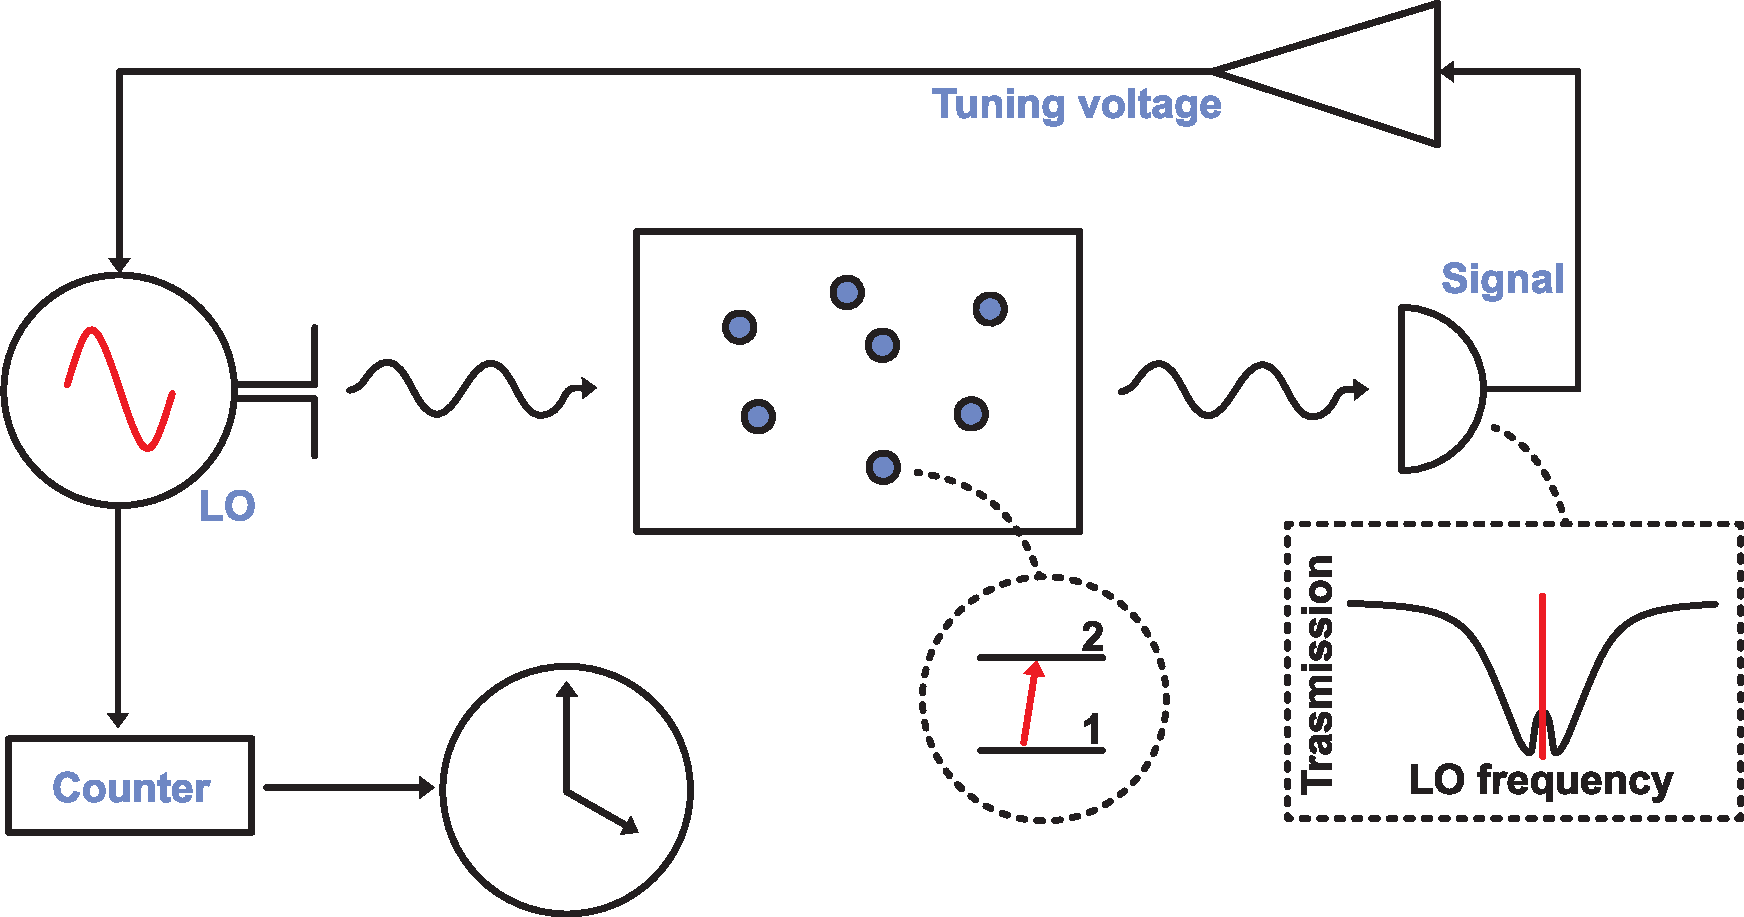
\includegraphics[width=0.7\textwidth, max width=\linewidth]{pdf/CSAC-scheme.pdf}
    \caption{General overview of a \acrshort{csac}}
    \label{fig:CSAC-general-overview}
\end{figure}

In the following sections, we will go through each main block of the \acrshort{csac}, highlighting their fundamental physics and explaining their role in the general framework of the clock.
In Section \ref{sec:performances_and_limitations}, all the limitations and bottleneck associated to each components will be discussed, analyzing their impact on the overall performance of the clock.

% \subsection{Physics Package (PP)}
\label{subsec:physics_package}

The \acrfull{pp} is the core component of the \acrshort{csac}, where the atomic excitation and interrogation take place.

Its function is to compare the frequency of the local oscillator with the atomic transition frequency and generate a signal that measures the difference between the two.
From a logical point of view, a generic PP receive as input the local oscillator frequency, and generate as output an electric signal that is sent to the control loop.
Electric power to excite the atoms and thermal power to maintain a steady temperature are also provided to the PP to ensure proper operation.

One of the keys in the stability of a \acrshort{csac}, lies in the capacity of the PP to generate a stable and accurate source of energy required for the excitation of the atoms, which leads to a stable and accurate signal for the control loop.

As we have mentioned at the beginning of this section (Section \ref{sec:working_principles}), \acrshort{csacs} can be divided into two main families based on the atomic element they use and the operating principle they follow.
In the following subsections (Subsections \ref{sssec:MODR} \& \ref{sssec:CPT}), we will delve into the specific architecture for the PP of the two main families of \acrshort{csacs}, namely the one based on \acrfull{modr} and the one based on \acrfull{cpt}.

\subsubsection{Microwave Optical Double-Resonance (MODR)}
\label{sssec:MODR}

In a \acrshort{pp} based on \acrfull{modr}, a vapor gas cell is irradiated simultaneously by a microwave signal (coming from the local oscillator) and a high frequency signal (coming from a laser source).
The combination of the two acting on the \acrfull{rb} atoms inside the cell allows understanding whether the local oscillator is in resonance with the atomic transition frequency or not.

In order to better visualize the operation of a MODR-based \acrshort{csac}, we leave here a schematic representation of its PP (Figure \ref{fig:MODR-physics-package-scheme}).

\begin{figure}[H]
    \centering
    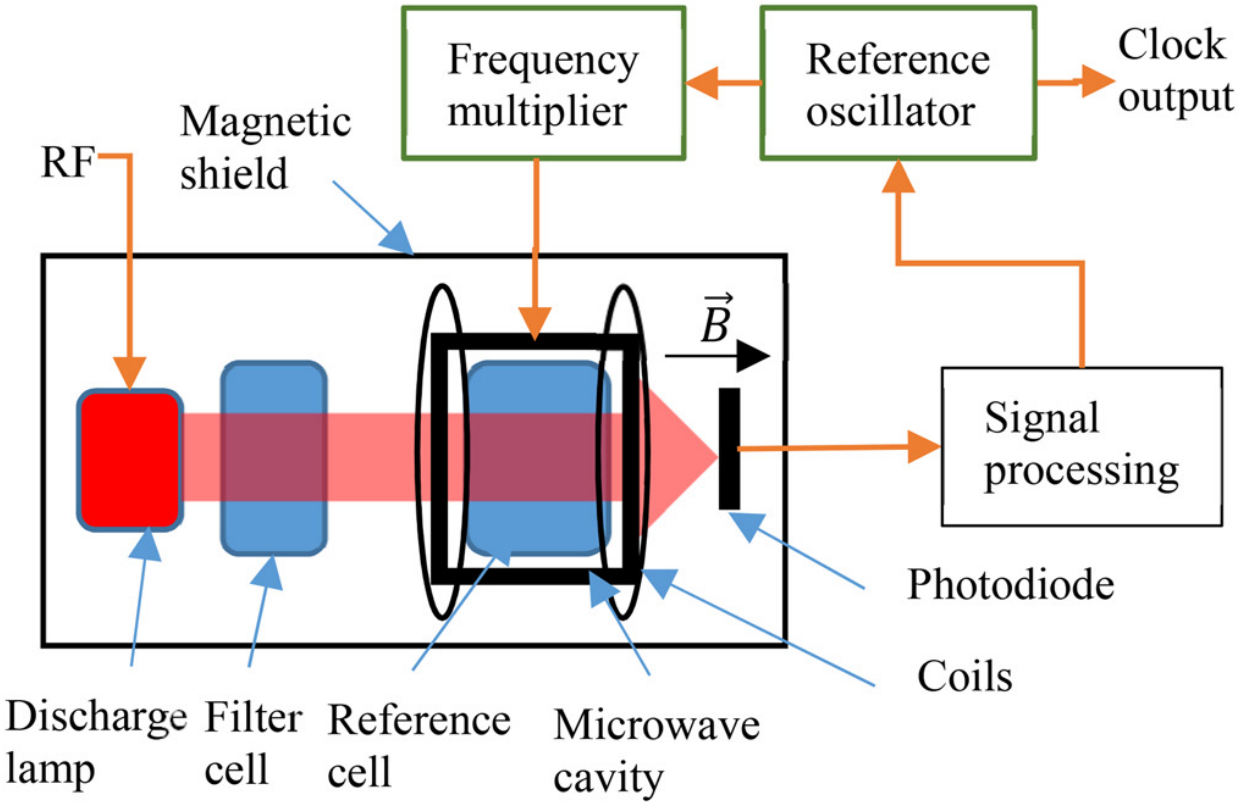
\includegraphics[width=0.6\textwidth, max width=\linewidth]{img/MODR-phisics-package-scheme.png}
    \caption{
        MODR-based \acrshort{csac} scheme.
        Source \cite{Kitching-2018}.
    }
    \label{fig:MODR-physics-package-scheme}
\end{figure}

\paragraph{Target Electron Transitions of Rubidium (Rb)}

In case of PP based on MODR, the vapor gas cell (also called reference cell) is typically filled with \acrfull{rb} ($^{87}Rb$) atoms.
$Rb$ is an alkaline metal with a relatively simple electronic structure, defined as $[Kr]5s^1$.
Its first ionization energy is $4.177 eV$, and the valence electron can be exited using relatively low energy photons.
For these reasons, $Rb$ is widely used in atomic clocks, as it allows for precise manipulation of the valence electron while containing the energy required for the excitation.

In particular, by recalling the quantum energy levels of $^{87}Rb$ (defined by quantum effects and interactions between the electron and the nucleus), we can better define our working frame for the MODR architecture.
Three different transitions are of interest regarding the $^{87}Rb$ atom\footnote{A more comprehensive analysis of the $5S$ \& $5P$ energy levels of $^{87}Rb$ can be found in the Appendix \ref{appendix:Rubidium-energy-levels}.}:

\begin{enumerate}[label = Rb.\Roman*, ref = Rb.\Roman*, leftmargin = *]
    \item \label{itm:Rb-I} $5^2S_{1/2} \quad F=1 \rightarrow 5^2S_{1/2} \quad F=2$: $\approx 6.8GHz$
    \item \label{itm:Rb-II} $5^2S_{1/2} \quad F=1 \rightarrow 5^2P_{1/2}$: $\approx 795^{-}nm$
    \item \label{itm:Rb-III} $5^2S_{1/2} \quad F=2 \rightarrow 5^2P_{1/2}$: $\approx 795^{+}nm$
\end{enumerate}

Notice that the transition $5^2S_{1/2} \rightarrow 5^2P_{1/2}$, of $\approx 795nm$, is usually refereed to as \textit{D1 line}.

As we will see in the following paragraphs, the only transitions that will excite the atoms in the reference cell are \ref{itm:Rb-I} and \ref{itm:Rb-II}.
Transition \ref{itm:Rb-III} is in fact a non-targeted transition that will be filtered out by the system before reaching the reference cell.


\paragraph{Pumping Source}

Having defined our working frame in terms of electron transitions of $^{87}Rb$, we can now step into understanding the mechanism used to excite the atoms in the reference cell.

In a MODR-based \acrshort{csac}, the pumping source is typically a \textit{bulb lamp} (also refereed to as \textit{discharge lamp}, see Figure \ref{fig:MODR-physics-package-scheme}) containing $^{87}Rb$ atoms that after being excited to a higher energy level by an external power source, they decay back to the ground energy level emitting photons.

Since there is no control over the pumping process inside the bulb lamp, more than one transition can be excited.
This means that the lamp will emit photons corresponding to different transitions of the $^{87}Rb$ atoms, including among the others \ref{itm:Rb-II} and \ref{itm:Rb-III} transitions.
However, the photons coming from the \ref{itm:Rb-III} transition are not of interest for the operation of the \acrshort{csac}, and they need to be filtered out.
To do so, a filter cell of $^{85}Rb$ is used since the transition energy of \ref{itm:Rb-III} is almost exactly the same as the transition energy $5^2P_{1/2} \quad F=3 \rightarrow 5^2P$ in $^{85}Rb$.

In the end, from the bulb lamp, the reference cell of the system will receive only photons associated with the \ref{itm:Rb-II} transition.


\paragraph{Electrons Excitation and Interrogation}

Having explained the excitation source, we can now proceed understanding how this energy is used over the atoms present in the \textit{reference cell} (see Figure \ref{fig:MODR-physics-package-scheme}, also refereed to as \textit{vapor gas cell}) and in particular what's the cycle that electrons are forced to.

For the simplicity of explanation, we will consider the different stages of the electrons as if they happen in a temporal sequence.
However, it's important to remind that these stages are not sequential but they happen simultaneously.

We can define three different stages in the cycle of the electrons:

\begin{itemize}
    \item Optical pumping (population inversion and decay): the laser source coming from the bulb lamp excites the atoms to a higher energy level and a population inversion is created between the two hyperfine states $5S_{1/2} F=1$ and $5S_{1/2} F=2$.
    \item Microwave excitation: the microwave signal coming from the local oscillator excites the atoms and, if it's in resonance with the \ref{itm:Rb-I} transition, it force the population accumulated in the $5S_{1/2} F=2$ state to fall back to the $5S_{1/2} F=1$ state.
    \item Optical pumping (interrogation): the same laser used for population inversion is now used to interrogate the atoms and understand if the microwave signal was in resonance with \ref{itm:Rb-I} transition or not.
\end{itemize}

To better understand the cycle of the electrons, we can refer to Figure \ref{fig:MODR-steps}.

\begin{figure}[H]
    \centering

    \begin{minipage}[t]{0.3\linewidth}
        \centering
        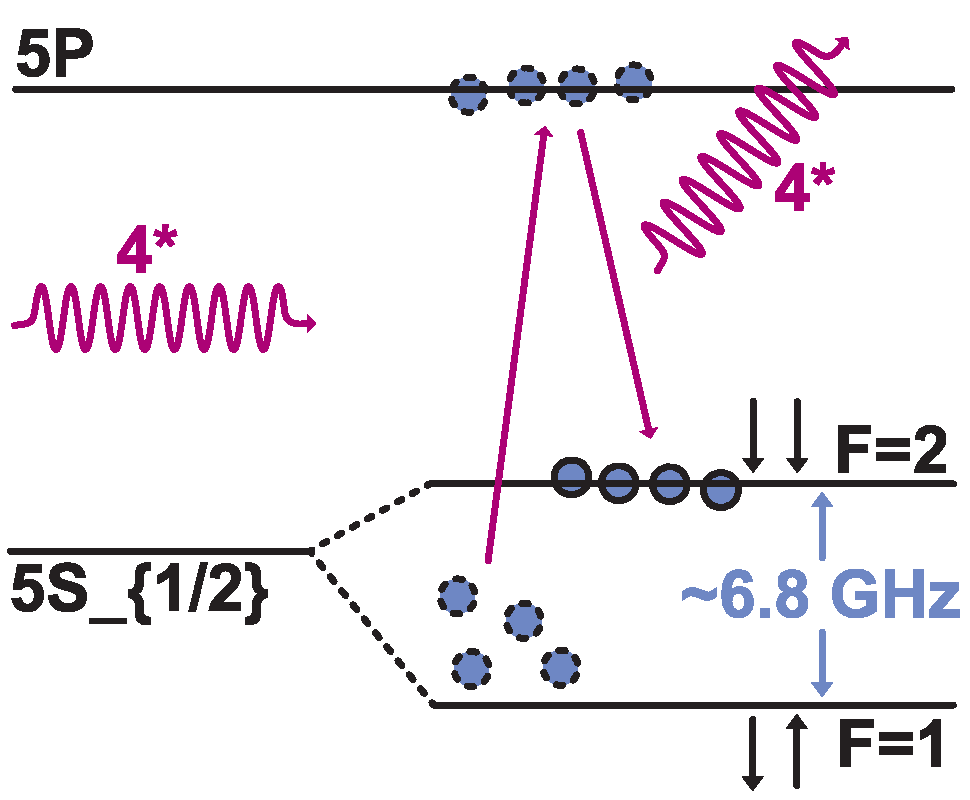
\includegraphics[width=\linewidth]{pdf/MODR/pumping-decay.pdf}
        \caption{Population inversion and decay.}
        \label{fig:MODR-pumping-decay}
    \end{minipage}
    %
    \hfill
    %
    \begin{minipage}[t]{0.3\linewidth}
        \centering
        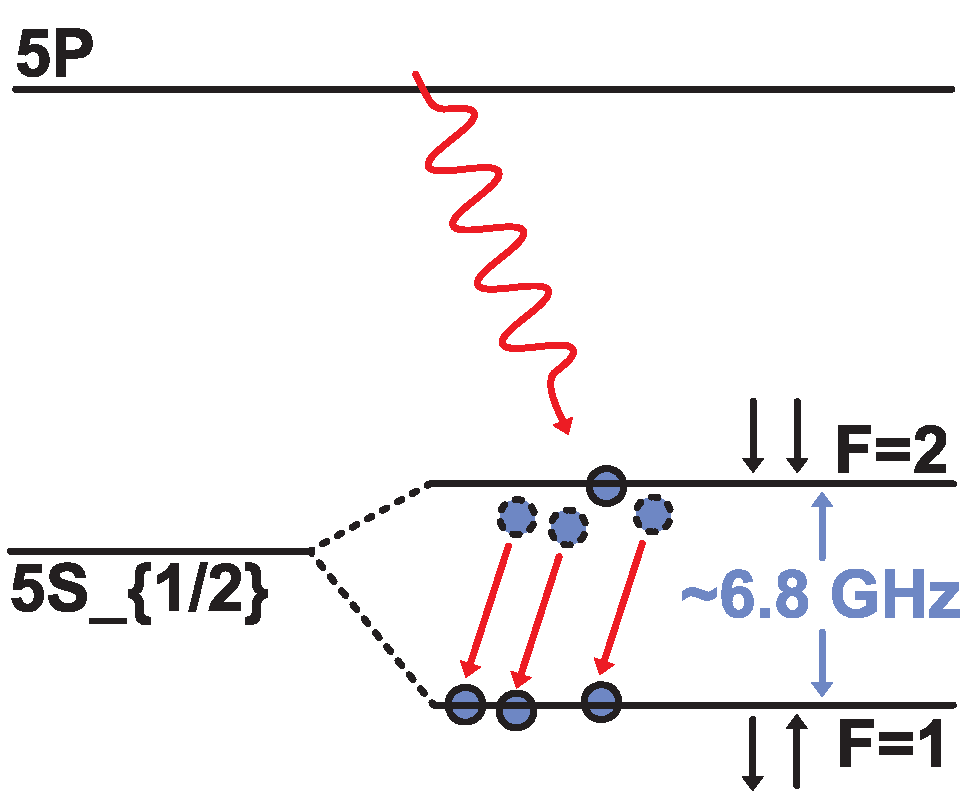
\includegraphics[width=\linewidth]{pdf/MODR/microwave.pdf}
        \caption{Microwave excitation.}
        \label{fig:MODR-microwave}
    \end{minipage}
    %
    \hfill
    %
    \begin{minipage}[t]{0.3\linewidth}
        \centering
        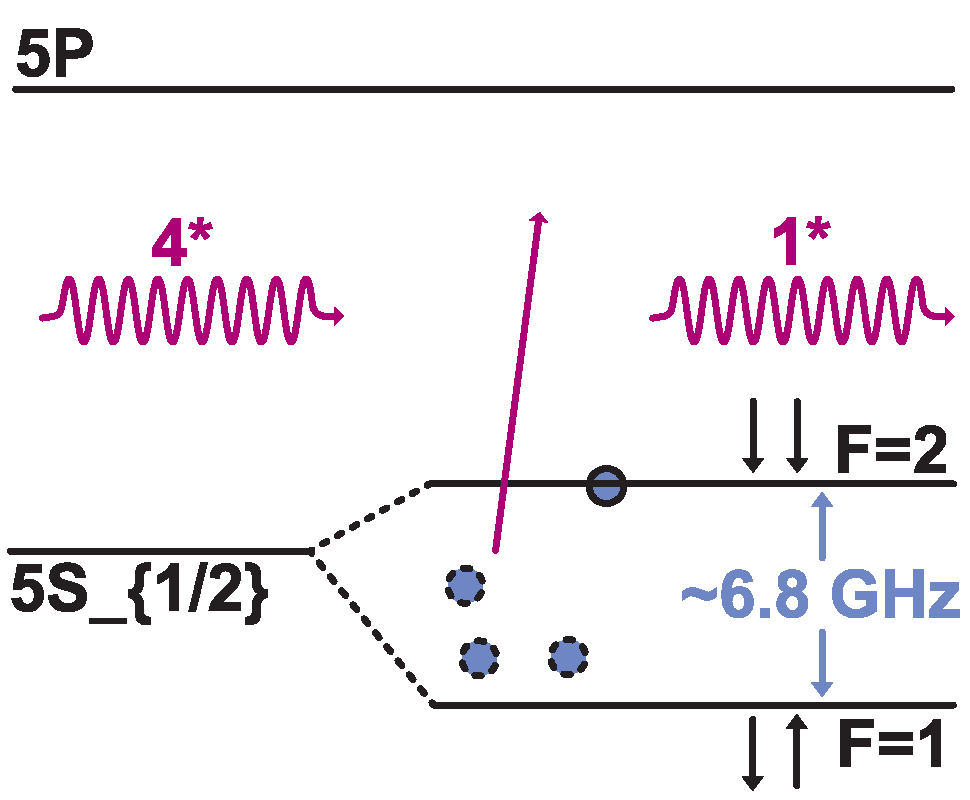
\includegraphics[width=\linewidth]{pdf/MODR/interrogation.pdf}
        \caption{Optical interrogation.}
        \label{fig:MODR-interrogation}
    \end{minipage}

    \caption{Electrons cycle in a MODR-based \acrshort{csac} due to the optical pumping, microwave excitation, and optical interrogation.}
    \label{fig:MODR-steps}
\end{figure}

With reference to Figure \ref{fig:MODR-steps}, we can now analyze deeper the different stages of the cycle and understand how it's possible to detect whether the microwave signal is in resonance with the atomic transition or not.

In particular, in Figure \ref{fig:MODR-pumping-decay} we can see four high energy photons coming from the pumping source that excite the electrons found at $5S_{1/2} F=1$, to $5^2P_{1/2}$ state.
From here, electrons will decay to both the $5^2S_{1/2} F=2$ and the $5^2S_{1/2} F=1$ states.
Over time however, the population will tend to accumulate on the $5^2P_{1/2} F=2$ state given that the excitation photons are not coupled with the \ref{itm:Rb-III} transition (due to the filter cell action).

During the second stage (Figure \ref{fig:MODR-microwave} for reference), the microwave excitation coming from the local oscillator is used to force the decay of the electrons from the $5^2S_{1/2} F=2$ state to the $5^2S_{1/2} F=1$ state.
Notice, however, that the decay is possible only if the microwave signal is at the right frequency of the transition, that is \ref{itm:Rb-I}.
In case the microwave signal is not exactly in resonance with the atomic transition, not all the electrons will be forced to decay and some of them will remain in the excited state.
Figure \ref{fig:MODR-microwave} shows an example where the microwave signal is not in perfect resonance with the atomic transition and 1 out of the 4 electrons remain in the $5^2S_{1/2} F=2$ state.

Finally, the cycle is closed with the interrogation phase (Figure \ref{fig:MODR-interrogation}).
Here, by sending the same amount of irradiation as in the pumping phase, we are able to detect if electrons are in the $5^2S_{1/2} F=1$ state or in the $5^2S_{1/2} F=2$ state.
In particular, in case not the entire population has decayed to the $5^2S_{1/2} F=1$ state during the microwave excitation, the interrogation phase will show a different intensity of the transmitted light.
In Figure \ref{fig:MODR-interrogation}, we can see that 1 out of the 4 photons will be transmitted given that only 3 atoms are in the $5^2S_{1/2} F=1$ state.

By measuring the intensity of the transmitted light, we can understand if the microwave signal was in resonance with the atomic transition or not.


\paragraph{Photodetector}

At the end of the vapor gas cell, a photodetector is used to measure the intensity of light transmitted through the reference cell.

In case of a MODR-based \acrshort{csac}, only if the microwave signal was in resonance with the atomic transition, most of the laser source from the bulb lamp will be absorbed by the atoms and the transmitted light will be minimal.
Conversely, in case of a non-resonant microwave signal, the intensity of the transmitted light will be stronger.

The signal captured by the photodetector is then sent to the control loop that will use it to fine-tune the local oscillator frequency.

\subsubsection{\acrfull{cpt}}
\label{sssec:CPT}

In case of a \acrfull{cpt} system, the physics package contains a vapor gas cell that receive a high energy signal from a laser source and force the valence electron of the \acrfull{cs} atoms to a coherent superposition of the two hyperfine ground states.
If this coherent superposition happens, the electron is said to be \textit{trapped in a dark state}, given that the incoming laser source will no more be coupled with the electron transitions and the atoms will not absorb the photons.

In a Physics Package based on \acrfull{cpt}, a vapor gas cell is irradiated by a highly modulated-circularly polarized laser source.
The laser source is modulated based on the local oscillator frequency.
Based on the effect of the laser source on the \acrfull{cs} atoms, we can understand whether the local oscillator is in resonance with the atomic transition frequency or not.

In order to better understand the operation of a CPT-based \acrshort{csac}, we leave here a schematic representation of its PP (Figure \ref{fig:CPT-physics-package-scheme}).

\begin{figure}[H]
    \centering
    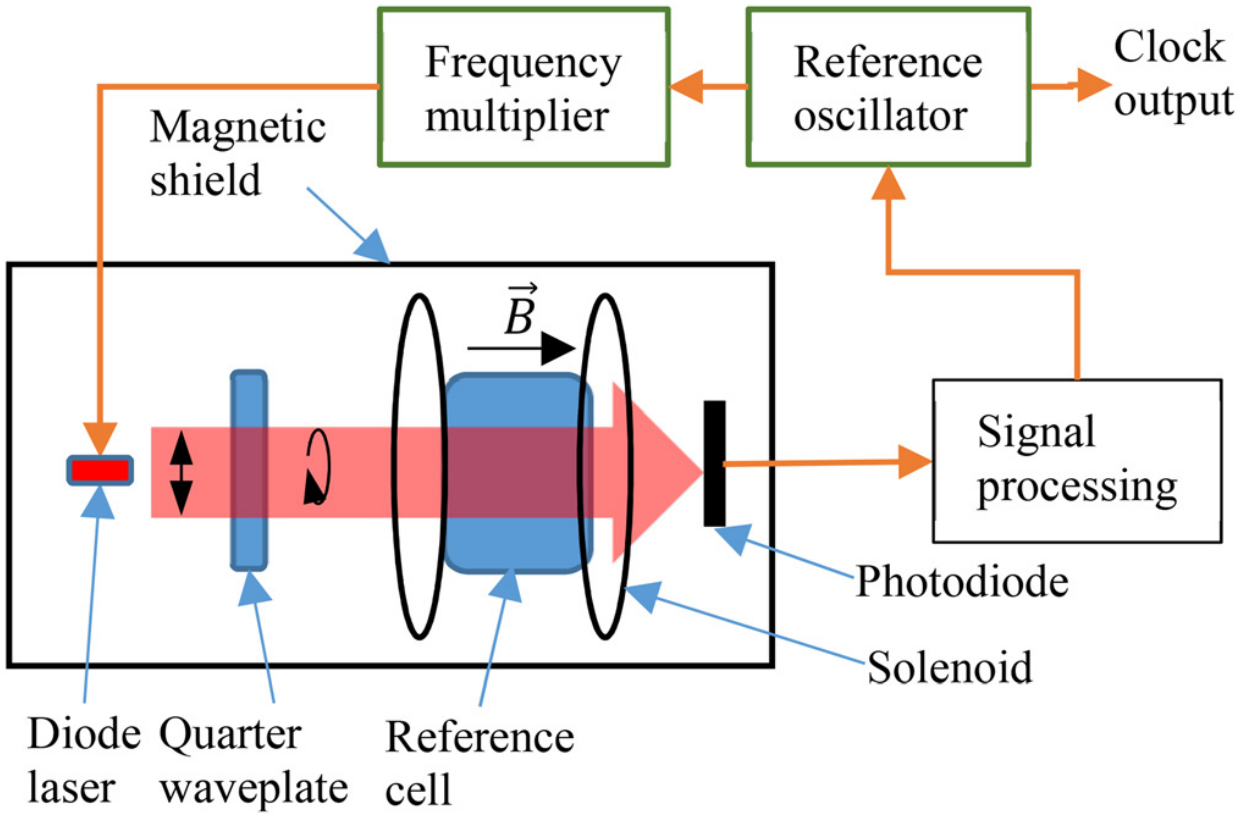
\includegraphics[width=0.6\textwidth, max width=\linewidth]{img/CPT-phisics-package-scheme.png}
    \caption{
        CPT-based \acrshort{csac} scheme.
        % Tha main components of the Physics Package are
    }
    \label{fig:CPT-physics-package-scheme}
\end{figure}

% MODR copy-paste
\paragraph{Target Electron Transitions of \acrfull{rb}}

In case of PP based on CPT, the vapor gas cell is typically filled with \acrfull{cs} ($^{133}Cs$) atoms.
$Cs$ is an alkaline metal with a relatively simple electronic structure, defined as $[Xe]6s^1$.
Its ionization energy is $3.894 eV$, and the valence electron can be exited using relatively low energy levels.
For these reasons, $Cs$ is widely used in atomic clocks, as it allows for precise manipulation of the valence electron while containing the energy required for the excitation.

In particular, by recalling the quantum energy levels of $^{133}Cs$ (defined by quantum effects and interactions between the electron and the nucleus), we can better define our working frame for the CPT architecture.
Three different transitions are of interest regarding the $^{133}Cs$ atom\footnote{In case of interest, a more comprehensive analysis of the $6S$ \& $6P$ energy levels of $^{133}Cs$ can be found in the Appendix \ref{appendix:Cesium-energy-levels}.}:

\begin{enumerate}[label = Cs.\Roman*, ref = Cs.\Roman*, leftmargin = *]
    \item \label{itm:Cs-I} $6^2S_{1/2} \quad F=3 \rightarrow 6^2S_{1/2} \quad F=4$: $\approx 9.2GHz$
    \item \label{itm:Cs-II} $6^2S_{1/2} \quad F=3 \rightarrow 6^2P_{1/2}$: $\approx 895^{-}nm$
    \item \label{itm:Cs-III} $6^2S_{1/2} \quad F=4 \rightarrow 6^2P_{1/2}$: $\approx 895^{+}nm$
\end{enumerate}

Notice that the transition $6^2S_{1/2} \rightarrow 6^2P_{1/2}$, of $\approx 895nm$, is usually refereed to as \textit{D1 line}.

\ref{itm:Cs-I}

\paragraph{Quantum Superposition}

Before moving on and understanding the different components of the CPT-based \acrshort{csac}, it's important to understand the concept of quantum superposition as it will be the key in the operation of the system.

In quantum mechanics, a quantum superposition is a fundamental principle that states that linear combinations of solutions to the Schr\"{o}dinger equation are also solutions of the Schr\"{o}dinger equation.
In other words, if $\ket{\psi_1}$ and $\ket{\psi_2}$ are solutions of the Schr\"{o}dinger equation, then $\alpha\ket{\psi_1} + \beta\ket{\psi_2}$ is also a valid solution of the state of the system.
A valid quantum superposition can be generally defined as:

\begin{equation}
    \ket{\psi} = c_\alpha\ket{\psi_\alpha} + c_\beta\ket{\psi_\beta}
\end{equation}

Where $\ket{\psi_\alpha}$ and $\ket{\psi_\beta}$ are two different states of the system and $c_\alpha$ and $c_\beta$ are complex numbers.
Practically speaking, this means that the electron can be found not only at the energy level associated with $\ket{\psi_\alpha}$ or $\ket{\psi_\beta}$, but also in a superposition of the two states (i.e. in any linear combination of the two states with a probability defined by the complex numbers).

To facilitate understanding of this counterintuitive concept, we report in the following two different interpretations of the quantum superposition:

\begin{itemize}
    \item Bloch Sphere representation: by imagining the electron as a 3D sphere with a finite radius, we can try to represent its energy level (i.e. its state) with a spatial vector with the origin in the center of the sphere and the tip on the surface. By mapping the ground state with an upward vector (Figure \ref{fig:Bloch-sphere-ground-state}) and the excited state with a downward vector (Figure \ref{fig:Bloch-sphere-excited-state}), we can intuitively understand that any other direction the vector might assume must be associated with a valid state of the electron. In other words, any other direction the state-vector other than the ground or the excited state is a valid quantum superposition that the electron can assume.
    \item Modal interpretation: given that to each energy level of the electron is associated a wave function, we can interpret the quantum superposition as a linear combination of the wave functions associated with the different energy levels. This interpretation derives from the approach used in classical vibrations problem, where the superposition of different modes (i.e. waves of different frequencies) can be used to describe the vibration of the system. In figure \ref{fig:modal-superposition}, we can see the superposition of two different modes that generate a new wave function.
\end{itemize}

\begin{figure}[H]
    \centering

    \begin{minipage}[t]{0.3\linewidth}
        \centering
        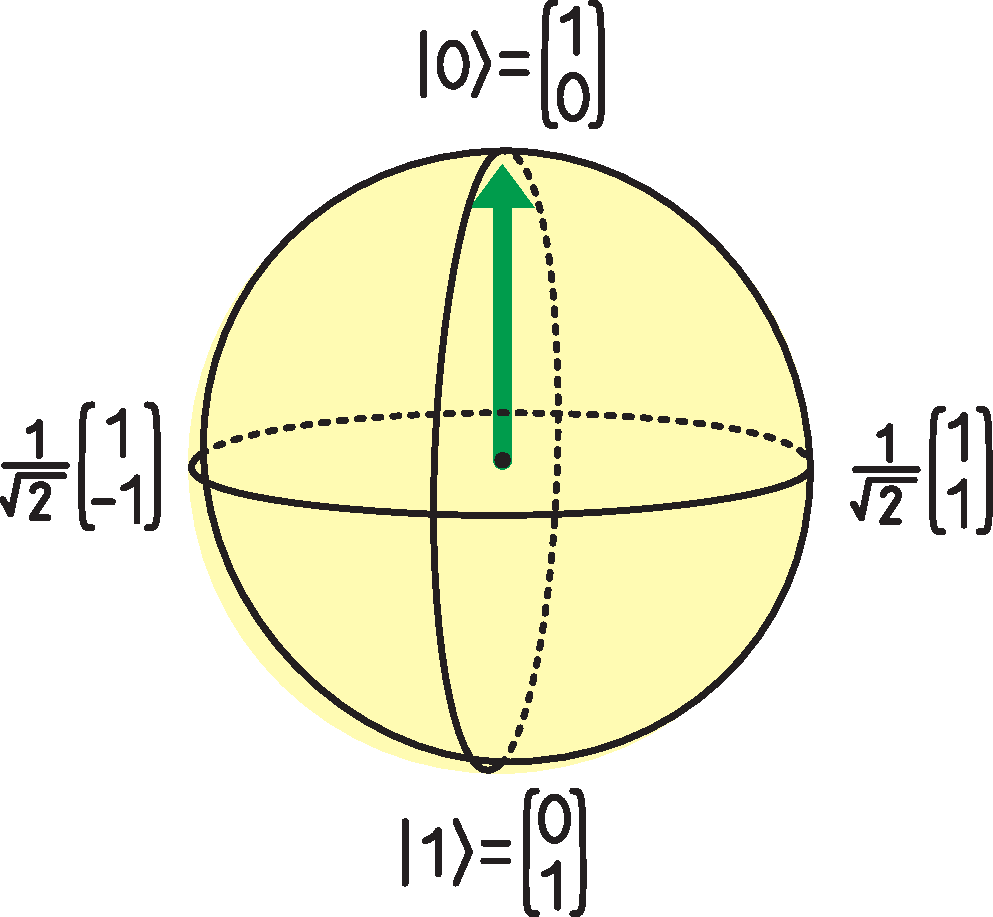
\includegraphics[width=\linewidth]{pdf/states/ground-state.pdf}
        \caption{Ground state.}
        \label{fig:Bloch-sphere-ground-state}
    \end{minipage}
    %
    \hfill
    %
    \begin{minipage}[t]{0.3\linewidth}
        \centering
        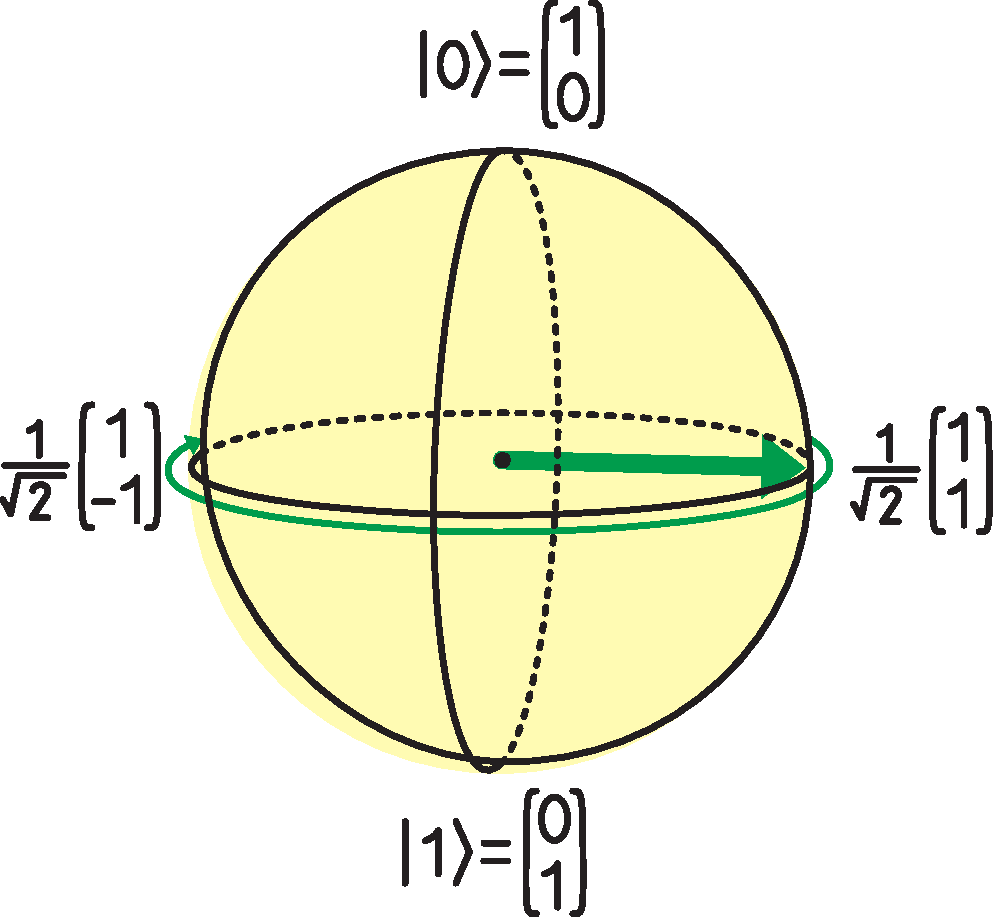
\includegraphics[width=\linewidth]{pdf/states/superposition-state.pdf}
        \caption{Superposition state.}
        \label{fig:Bloch-sphere-superposition}
    \end{minipage}
    %
    \hfill
    %
    \begin{minipage}[t]{0.3\linewidth}
        \centering
        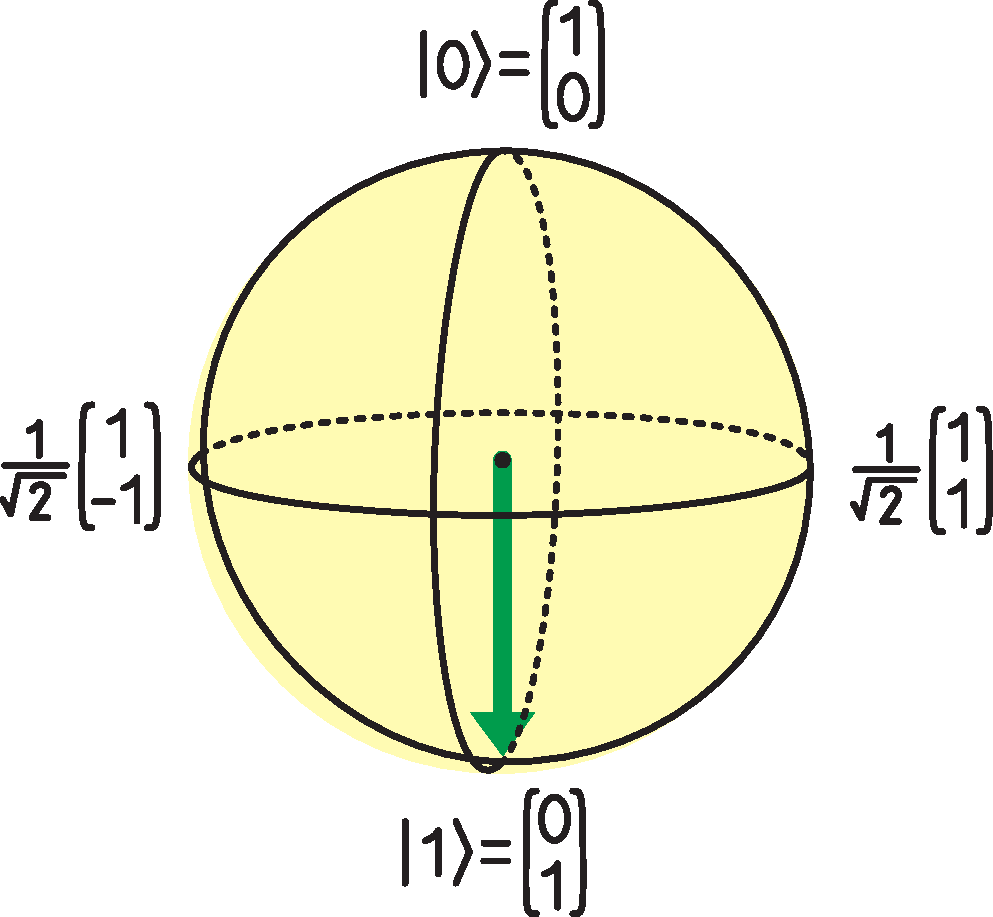
\includegraphics[width=\linewidth]{pdf/states/excited-state.pdf}
        \caption{Excited state.}
        \label{fig:Bloch-sphere-excited-state}
    \end{minipage}

    \caption{State superposition via Bloch sphere representation.}
    \label{fig:Bloch-sphere}
\end{figure}

\begin{figure}[H]
    \centering

    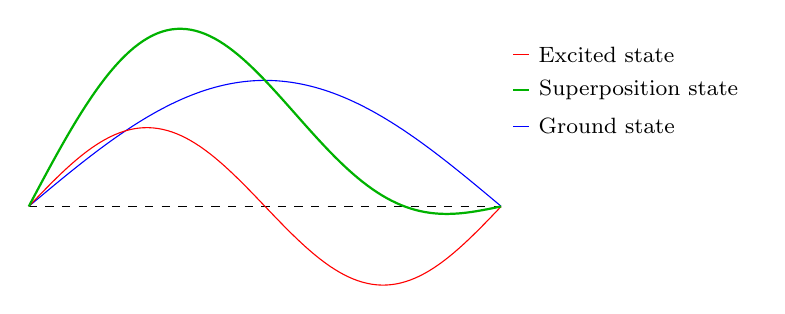
\begin{tikzpicture}

        \draw[dashed] (0, 0) -- (6, 0);

        \draw[blue, domain=0:6, samples=100] plot (\x, {1.6*sin(180/6*\x)});
        \draw[red, domain=0:6, samples=100] plot (\x, {1.0*sin(360/6*\x)});
        \draw[green!70!black, thick, domain=0:6, samples=100] plot (\x, {1.6*sin(180/6*\x) + 1.0*sin(360/6*\x)});

        % Add legend
        \node [matrix, font = \footnotesize, below right, row sep = 0cm] at (current bounding box.north east)
        {
            \draw[red] (0, 0) -- ++(0.2, 0) node[right, black] {Excited state}; \\
            \draw[green!70!black, thick] (0, 0) -- ++(0.2, 0) node[right, black] {Superposition state}; \\
            \draw[blue] (0, 0) -- ++(0.2, 0) node[right, black] {Ground state}; \\
        };

    \end{tikzpicture}

    \caption{State superposition via modal interpretation and wave functions.}
    \label{fig:modal-superposition}
\end{figure}


\paragraph{$\Lambda$-Lambda System \& Dark State}

Having understood the concept of quantum superposition, we can proceed and understand how it's useful related to the operation of a CPT-based \acrshort{csac}.
To do so, we need to introduce the concept of $\Lambda$-Lambda system and dark state.

A $\Lambda$-Lambda system is a quantum system composed of three energy levels (see Figure \ref{fig:lambda-system} for reference), where not all the dipole transitions are allowed.
In particular:

\begin{figure}[H]
    \centering

    \begin{minipage}[c]{0.49\linewidth}
        \centering
        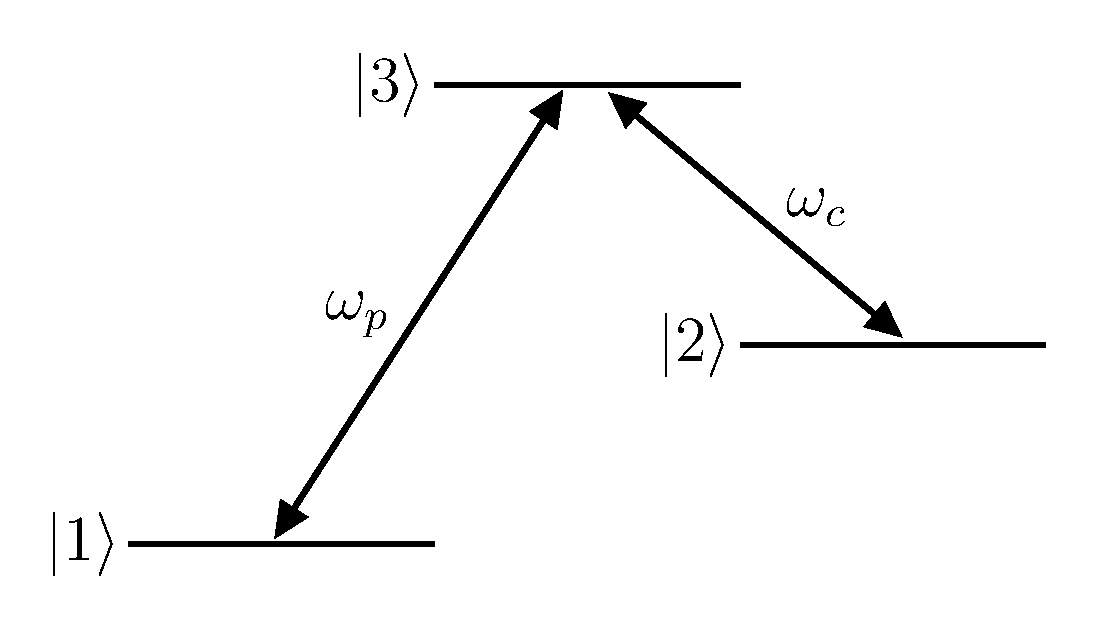
\includegraphics[width=\textwidth, max width=\linewidth]{pdf/lambda-system.pdf}
        \caption{$\Lambda$-system representation.}
        \label{fig:lambda-system}
    \end{minipage}
    %
    \hfill
    %
    \begin{minipage}[c]{0.49\linewidth}
        \begin{align}
            \text{Allowed transitions:}  & \begin{cases}
                                               \ket{1} \leftrightarrow \ket{3} \\
                                               \ket{2} \leftrightarrow \ket{3}
                                           \end{cases} \\
            \text{Forbidden transition:} & \begin{cases}
                                               \ket{1} \leftrightarrow \ket{2}
                                           \end{cases}
        \end{align}
    \end{minipage}

\end{figure}


In case the system is excited with a stable and well-controlled laser source (better explanation given in the following paragraph) that couples at the same time both the $\ket{1} \leftrightarrow \ket{3}$ and the $\ket{2} \leftrightarrow \ket{3}$ transitions, electrons will be pumped at first in their excited state (i.e. $\ket{3}$) and then forced to decay to $\ket{\psi}$, a superposition of $\ket{1}$ and $\ket{2}$.
This method is called \textit{coherent population trapping} and the system is said to be in a \textit{dark state} given that the incoming laser source will no more be coupled with the electron transitions and the atoms will not absorb the photons.

In our working frame, the $\Lambda$-system is composed of the two ground states $6^2S_{1/2} F=3$ \& $6^2S_{1/2} F=4$ and the excited state $6^2P_{1/2}$ of the $^{133}Cs$ atom.


\paragraph{Pumping Source}

From now on, given for granted the concept of quantum superposition and the $\Lambda$-system, we can step into understanding the components used to excite the $^{133}Cs$ atoms and obtain the desired dark state.

In a CPT-based \acrshort{csac}, the pumping source is typically a \textit{diode laser} (see Figure \ref{fig:CPT-physics-package-scheme} for reference), and most commonly a \textit{Vertical Cavity Surface Emitting Laser (VCSEL)}.
The use of a diode laser instead of a bulb lamp is due to the need of a stable and well-controlled source of irradiation that can be precisely modulated based on the local oscillator frequency.
In fact, VCSEL is a semiconductor laser diode that emits light from its top surface and it's characterized by a very narrow emission spectrum and a high modulation bandwidth.

In the framework of a CPT-based \acrshort{csac}, the diode laser is driven by the local oscillator frequency and it's modulated in both Amplitude (AM) and Frequency (FM).
In particular, in order to obtain the desired effect of coherent population trapping inside the reference cell, the laser source must met the following requirements:

\begin{itemize}
    \item AM modulation: the signal generated via the AM modulation must be at frequency \ref{itm:Cs-I} (i.e. the transition frequency of the $^{133}Cs$ ground states hyperfine splitting);
    \item FM modulation: the signal generated via the FM modulation must be at frequency of the \textit{D1 line} (i.e. the transition frequency of the $^{133}Cs$ ground state to the $^{133}Cs$ excited state).
    \item Circular polarization: the laser source must be positively circularly polarized.
\end{itemize}

The first two requirements can be easily met by controlling the injection current of the diode laser in time and are equivalent to state that the laser source must be the sum of a signal modulated at \ref{itm:Cs-II} with another modulated at \ref{itm:Cs-III} frequency.
In other words, the laser source must be able to generate the beating wave of the two frequencies as shown in Figure \ref{fig:beating-wave}.
The third requirement can be met by using a quarter-wave plate in front of the laser source that convert the linear polarization of the source in a circular one (again, see Figure \ref{fig:CPT-physics-package-scheme} for reference).

\begin{figure}[H]
    \centering

    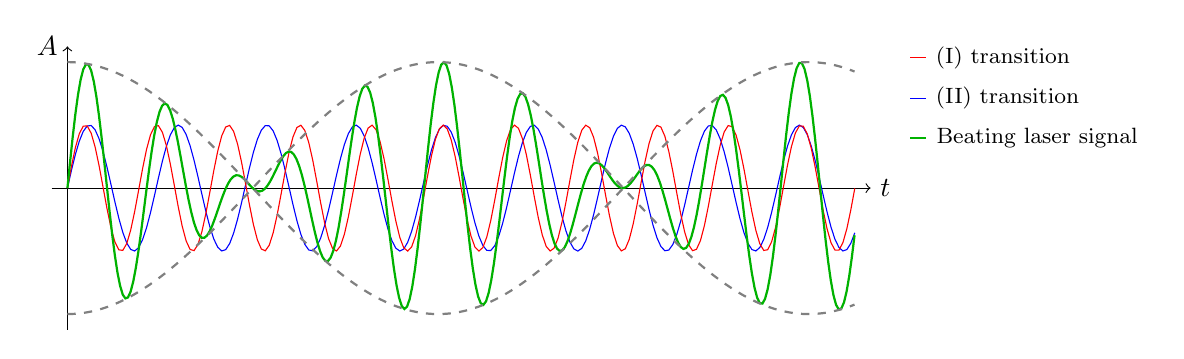
\begin{tikzpicture}
        \def\fa{1.775/2}
        \def\fb{2.20/2}
        \def\xmax{10}

        \draw[->] (-0.2, 0) -- (\xmax + 0.2, 0) node[right] {$t$};
        \draw[->] (0, -1.8) -- (0, 1.8) node[left] {$A$};

        \draw[blue, domain=0:\xmax, samples=200] plot (\x, {0.8*sin(360*\fa*\x)});
        \draw[red, domain=0:\xmax, samples=200] plot (\x, {0.8*sin(360*\fb*\x)});
        \draw[green!70!black, thick, domain=0:\xmax, samples=300] plot (\x, {0.8*sin(360*\fa*\x) + 0.8*sin(360*\fb*\x)});
        \draw[gray, thick, dashed, domain=0:\xmax, samples=300] plot(\x,{ 1.6*cos(180*(\fa-\fb)*\x)});
        \draw[gray, thick, dashed, domain=0:\xmax, samples=300] plot(\x,{ -1.6*cos(180*(\fa-\fb)*\x)});

        % Add legend
        \node [matrix, font = \footnotesize, below right, row sep = 0cm] at (current bounding box.north east)
        {
            \draw[red] (0, 0) -- ++(0.2, 0) node[right, black] {\textrm{(I)} transition}; \\
            \draw[blue] (0, 0) -- ++(0.2, 0) node[right, black] {\textrm{(II)} transition}; \\
            \draw[green!70!black, thick] (0, 0) -- ++(0.2, 0) node[right, black] {Beating laser signal}; \\
        };

    \end{tikzpicture}

    \caption{Beating wave of the laser source in a CPT-based \acrshort{csac} (AM modulation is highlighted with a dashed gray line, FM modulation is clearly visible on the green wave).}
    \label{fig:beating-wave}
\end{figure}

Notice, however, that the one represented in Figure \ref{fig:beating-wave} is the ideal case where the laser source is perfectly modulated at the two frequencies \ref{itm:Cs-II} and \ref{itm:Cs-III}.
In reality, the laser source is driven by the local oscillator frequency and some modulation errors will appear.
Those shift with respect to the ideal case will give us the information needed to understand if the local oscillator is in resonance with the atomic transition or not (i.e. if the local oscillator is at the right frequency or not).

\paragraph{Electrons Excitation and Interrogation}

Having understood what is the excitation source, we can now proceed understanding how this energy is used over the atoms present in the \textit{reference cell} (see Figure \ref{fig:CPT-physics-package-scheme}, also refereed to as \textit{vapor gas cell}) and in particular what's the cycle that electrons are forced to.

For the simplicity of the explanation, we will consider the different stages of the electrons as if they happen in a temporal sequence.
However, it's important to remind those stages are not sequential but they simultaneously happen.

We can define three different stages in the cycle of the electrons:

\begin{itemize}
    \item Optical pumping (population inversion): the laser source coming from the diode laser excites the atoms from both the $6S_{1/2} F=3$ and the $6S_{1/2} F=4$ ground hyperfine states to the $6^2P_{1/2}$ excited state.
    \item Decay to the dark state (superposition state): if the laser source during the pumping stage is modulated properly as described in the previous paragraph, then the excited electrons will now decay to a coherent superposition of the two ground states $6S_{1/2} F=3$ and $6S_{1/2} F=4$. The atoms are now in a dark state.
    \item Optical pumping (interrogation): the same laser used for population inversion is now used to interrogate the atoms and understand if the local oscillator frequency was in resonance with the atomic transition \ref{itm:Cs-I} or not.
\end{itemize}

To better understand the cycle of the electrons, we can refer to Figure \ref{fig:CPT-steps}.

\begin{figure}[H]
    \centering

    \begin{minipage}[t]{0.3\linewidth}
        \centering
        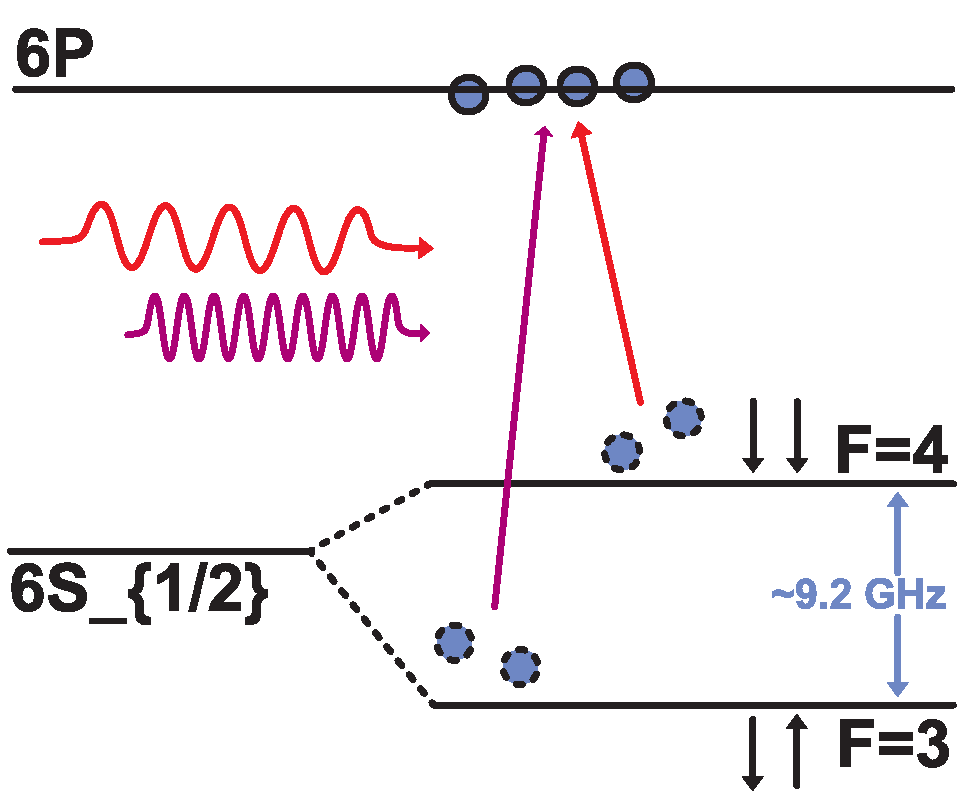
\includegraphics[width=\linewidth]{pdf/CPT/pumping.pdf}
        \caption{Population inversion.}
        \label{fig:CPT-pumping}
    \end{minipage}
    %
    \hfill
    %
    \begin{minipage}[t]{0.3\linewidth}
        \centering
        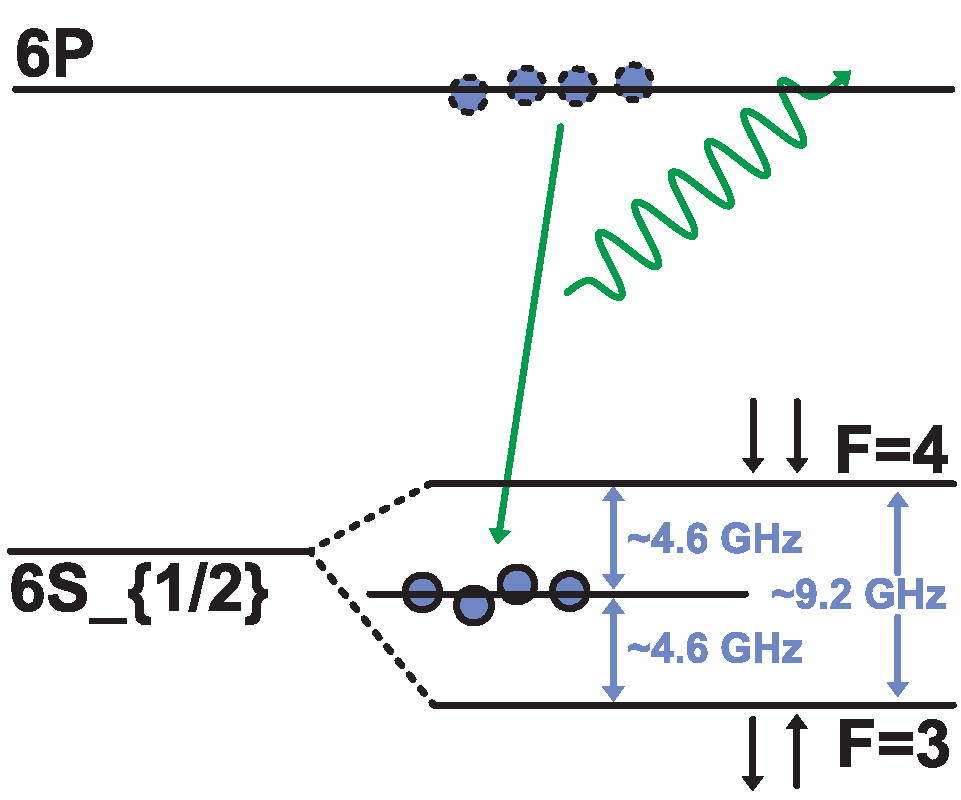
\includegraphics[width=\linewidth]{pdf/CPT/decay.pdf}
        \caption{Population decay.}
        \label{fig:CPT-decay}
    \end{minipage}
    %
    \hfill
    %
    \begin{minipage}[t]{0.3\linewidth}
        \centering
        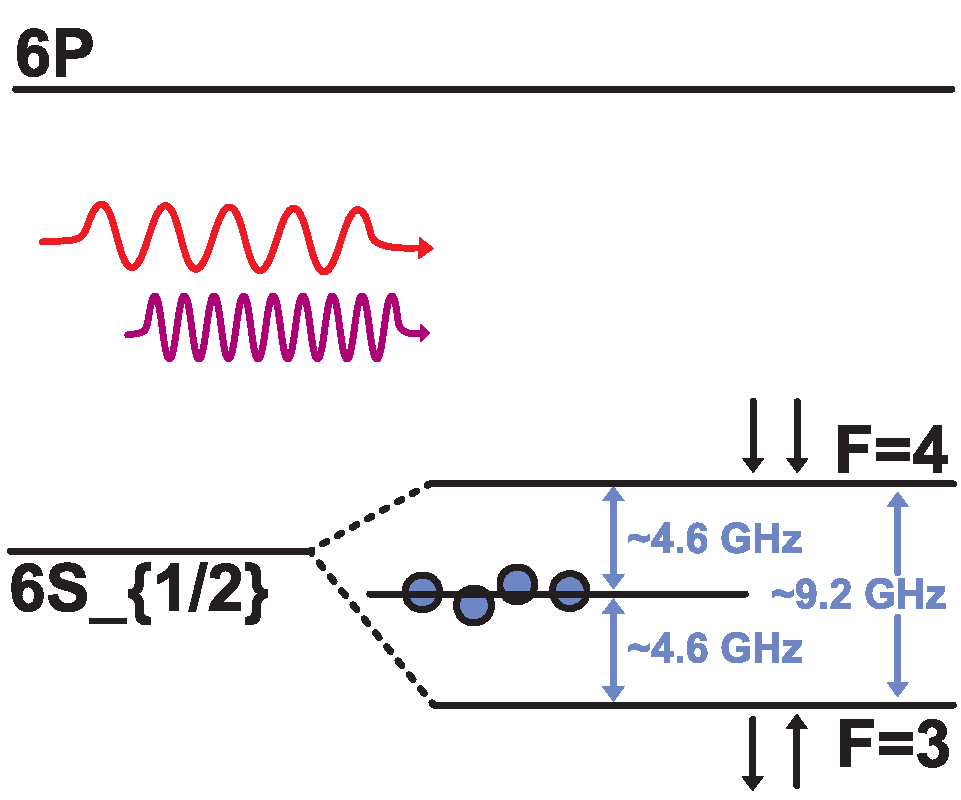
\includegraphics[width=\linewidth]{pdf/CPT/interrogation.pdf}
        \caption{Optical interrogation.}
        \label{fig:CPT-interrogation}
    \end{minipage}

    \caption{Electrons cycle in a CPT-based \acrshort{csac} due to the optical pumping, decay and optical interrogation.}
    \label{fig:CPT-steps}
\end{figure}

With reference to Figure \ref{fig:CPT-steps}, we can now analyze deeper the different stages of the cycle and understand how it's possible to detect whether the local oscillator is in resonance with the atomic transition or not.

For the sake of the explanation and simplification, we will consider the pumping laser source (the on coming from the diode laser) as two separate signals: one modulated at the frequency of the transition \ref{itm:Cs-II} and the other modulated at the frequency of the transition \ref{itm:Cs-III}.
In reality, the laser source is a beating wave of the two frequencies as shown in Figure \ref{fig:beating-wave}.
In Figure \ref{fig:CPT-pumping}, we can see four electrons that get excited from the $6S_{1/2} F=3$ and the $6S_{1/2} F=4$ ground hyperfine states to the $6^2P_{1/2}$ excited state.

Being $6^2P_{1/2}$ an unstable state, the electrons will start to decay to the non-excited states.
However, if the pumping laser source was modulated properly during the pumping stage, the electrons will now start to decay not only to both $6S_{1/2} F=3$ and $6S_{1/2} F=4$ states, but also to superposition state of the two.
In Figure \ref{fig:CPT-decay}, we can see that over time the population will tend to accumulate in a coherent superposition of the two ground states, given that from here the electrons won't be excited by the laser source and are said to be trapped.
Notice however, that the accumulation in the superposition state is possible only if the laser source was pumping at the right frequency, that is equivalent to say that the local oscillator was in resonance with the atomic transition \ref{itm:Cs-I}.

Finally, the cycle is closed with the interrogation phase (Figure \ref{fig:CPT-interrogation}).
Here, by sending the same amount of irradiation as in the pumping phase, we are able to detect if electrons are in one of the two ground states or in the superposition state.
In particular, in case not the entire population has decayed to the dark state during the decay, the interrogation phase will show a different intensity of the transmitted light.
In Figure \ref{fig:CPT-interrogation}, we can see that all the electrons are found in the superposition state and so the intensity of the transmitted light will be maximal since none of those electrons is coupled with the laser source.

By measuring the intensity of the transmitted light, we can understand if the local oscillator was in resonance with the atomic transition or not.


\paragraph{Photodetector}

At the end of the reference cell, a photodetector is used to measure the intensity of light transmitted through it.

In case of a CPT-based \acrshort{csac}, given that if the microwave signal was in resonance with the atomic transition, most of the laser source from the diode laser won't be anymore coupled to any electron, then the intensity of the transmitted light will be maximal.
Conversely, in case of a non-resonant microwave signal, the intensity of the transmitted light will be lower given that a fraction of the light will be absorbed by the electrons that are not in the superposition state.
In Figure \ref{fig:CPT-transmission}, we can see an example of a detuned signal captured by the photodetector.

\begin{figure}[H]
    \centering
    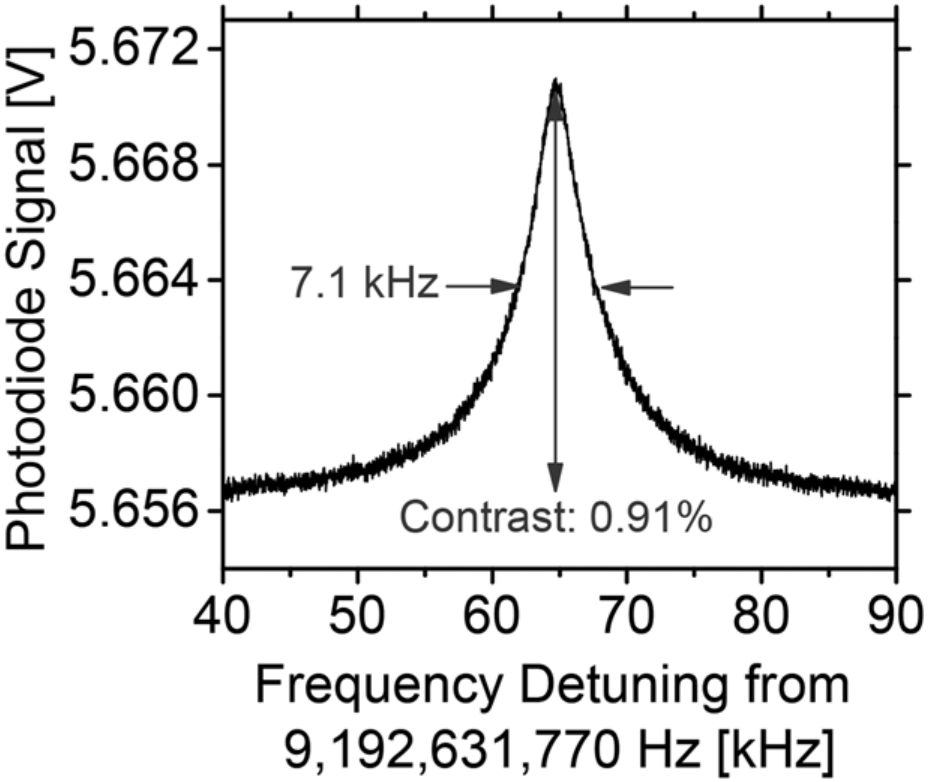
\includegraphics[width=0.5\textwidth, max width=0.8\linewidth]{img/CPT-transmission-signal.png}
    \caption{Detuned photodetection signal in a CPT-based \acrshort{csac}.}
    \label{fig:CPT-transmission}
\end{figure}

The signal captured by the photodetector is then sent to the control loop that will use it to fine-tune the local oscillator frequency (i.e. the clock frequency).


% TODO
\paragraph{Architecture Limitations}

Finally, we can move on and highlight the main limitations of a CPT-based \acrshort{csac} based on the metrics we have defined in Section \ref{sec:objective_metrics}.



\subsection{Control Loop (CL)}
\label{subsec:control_loop}

The \acrfull{cl} act as the brain of the clock, adjusting dynamically various parameters inside the \acrshort{csac} architecture to optimize stability and output frequency accuracy.
To do so, multiple servo loops based on PI\footnote{Proportional Integral} controllers are implemented to control specific areas and properties of different components. \acrshort{cl} takes as input the signal coming from the \acrfull{pp} and other sampled quantities coming from a network of sensors that are used to monitor the state of the clock (e.g., temperature sensors, magnetic field sensors, etc.)

\begin{figure}[H]
    \centering
    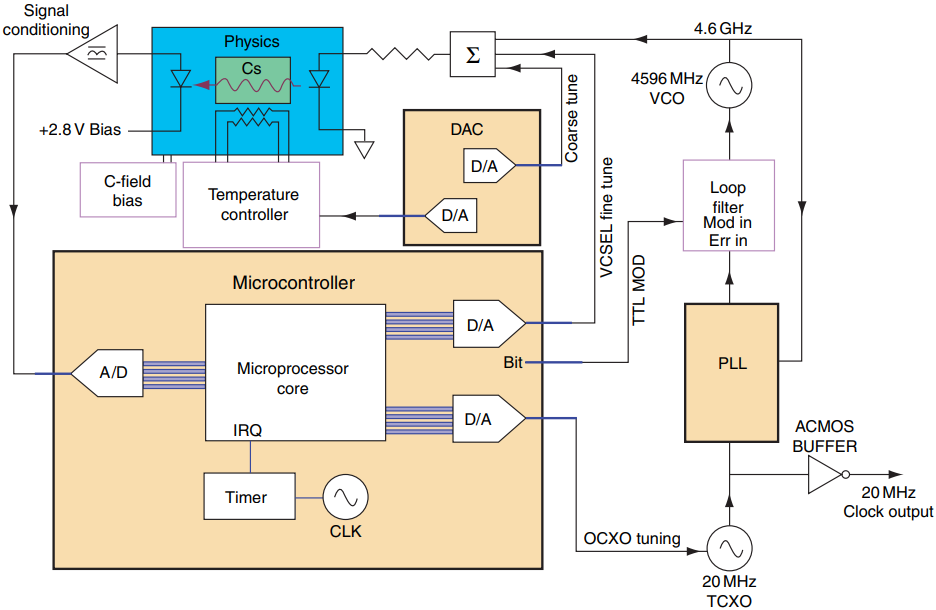
\includegraphics[width=.7\textwidth, max width=\linewidth]{img/control-loop.png}
    \caption{Control Loops block diagram for a CPT-based architecture (note the presence of the VCSEL). Source \cite{Knappe}.}
    \label{fig:control-loop}
\end{figure}

In Figure \ref{fig:control-loop} some key components are highlighted, such as microcontroller, converters (DAC and ADC), and PLL (Phase-Locked Loop) that are crucial for the correct functioning of the \acrshort{cl}.
In particular, the PLL is responsible for keeping in phase the \acrshort{lo} (indicated by the label "TCXO" in the bottom right) with the \acrshort{fs}, minimizing the phase noise and the frequency drift between the two components.

In a regular architecture, at least four servo loops are implemented to target different parameters.


\paragraph{Local Oscillator frequency servo loops}

The most important task of the \acrshort{cl} is the discipline of the \acrfull{lo} frequency to the desired value, locking it to the atomic resonance frequency or one of its multiple harmonics.

To achieve this, the \acrshort{cl} receives the output signal from the \acrshort{pp} and generate a feedback voltage signal that is sent to the \acrshort{lo} group.
Here, it's converted in a temperature variation of the crystal in order to modify its mechanical properties, thus adjusting the output frequency.

With reference to Figure \ref{fig:control-loop}, we can see this control line in the bottom right corner of the image, associated with the label "OCXO tuning", going from the microcontroller unit to the \acrshort{lo} group.

It has to be noted that the \acrshort{lo} has a much slower dynamics with respect to the electrical one provided by the microcontroller.
This causes an unavoidable delay over the feedback loop action and the actual effect on the \acrshort{lo} output frequency.


\paragraph{Laser frequency servo loops}

In case of the use of VCSEL as the excitation source, the \acrshort{cl} is also responsible for the control and tuning of its frequency that can be affected by external factors such as temperature variations or electrical/magnetic disturbances.

The diode laser is controlled by the summation of three different signal (see Figure \ref{fig:control-loop}), that are the coarse tune, the fine tune, and the \acrshort{fs} output.

In particular, the coarse tune signal is independent of any state of the clock and doesn't vary during the operation time.
The fine tune instead, is generated by the microcontroller and is used to compensate the environmental effects that cause a drift in the frequency of the excitation source.
Finally, the \acrshort{fs} output is added in order to permit the \acrshort{pp} to understand if the \acrshort{lo} is locked to the atomic resonance frequency.


\paragraph{Laser and cell temperature servo loops}

Maintaining constant temperatures for the laser and the reference cell within the \acrshort{pp} is another job of the \acrshort{cl}.

As we will see in the next section (Section \ref{sec:performances_and_limitations}), the temperature of these two components are crucial for the performances of the clock and should be maintained at a constant value during the operation time.

To do so, the feedback loop modify the temperature based on the signal coming from a network of thermocouple sensors that are placed near the targets.
Notice how, depending on the specific architecture of the clock, the \acrshort{cl} can act on the temperature of the two components independently or together.

In this way, the \acrshort{cl} ensures that both the excitation source and the atomic resonance frequencies are not affected by temperature variations, improving the photons coupling effectiveness.


\paragraph{Other servo loops}

In addition, other control loops can be implemented to target other parameters that might affect the performances of the clock.

Among these, one of particular importance is the servo used to shield or more in general control the magnetic field surrounding the \acrshort{pp}.
Again, with reference to Figure \ref{fig:control-loop}, we can recognize this control line in the bottom left corner of the "Physics" package block, associated with the label "C-field bias".

This control loop is used to maintain a zero or a constant value of the magnetic field inside the \acrshort{pp}, ensuring a precise and predictable behavior of the atomic resonance frequency that otherwise might suffer from frequency shifts (Zeeman and Stark effects, see Section \ref{sec:performances_and_limitations}).

\subsection{\acrfull{lo}}
\label{subsec:local_oscillator}
% \input{src/04 - performance}
% \section{Applications}
\label{sec:applications}

As we have seen in Section \ref{sec:performances_and_limitations}, the performance of a \acrshort{csac} varies depending on multiple factors that modify the nominal behavior of the internal components and the overall functionality of the clock.

However, the possibility of choosing components with different characteristics and the flexibility of the design, allows \acrshort{csac} to be used in a wide range of applications.
In the following, we will give an overview of the main applications that relies on \acrshort{csac} technology highlighting the requirements and the role the clock has in the application.
Here, applications are listed in order of their impact on society, starting from the most commonly used to the most specialized ones.

\subsection{Global Navigation Satellite System (GNSS)}
\label{subsec:GNSS}

The Global Navigation Satellite System (GNSS) is a satellite-based system that delivers geolocation and time information to any GNSS receiver that is able to receive contemporaneously signals from multiple satellites.
The GNSS system is adopted in a wide range of networks and applications, including the Global Positioning System (GPS), Galileo\footnote{The European alternative to the American GPS}, GLONASS\footnote{The Russian alternative to the American GPS}, and it is used in military, scientific, and commercial applications.
Basically, every application that requires a precise time reference and/or a precise position retrieve the information from the GNSS system.

The process used to calculate the position of the receiver is based on the \textit{trialateration} method, which compute the distance between the receiver and the satellites by measuring the time of the light signal to travel from the sender to the receiver.
Theoretically, the position of the receiver can be calculated by using the signals from three satellites, but in practice, a fourth satellite is used to correct the time offset of the receiver's clock.
In fact, under a mathematical point of view, the system to be solved is composed of four equations and four unknowns, where the unknowns are the position of the receiver in space and the time offset of the receiver's clock.

\begin{equation}
    \Delta d_i = c \cdot (\Delta t_i + \delta t) = \sqrt{(x_r - x_i)^2 + (y_r - y_i)^2 + (z_r - z_i)^2}, \quad i = 1, 2, 3, 4
\end{equation}

\begin{equation}
    \underbrace{x_r, y_r, z_r, \delta t}_\text{4 Unknowns requires 4 satellites}
\end{equation}


\paragraph{Role of CSAC}

Nowadays, the GNSS receiver usually uses a quartz crystal oscillator to generate the clock signal.
However, this type of oscillator has a high drift rate, which means that the time offset of the receiver's clock can change significantly over time.
This is also the reason why the fourth satellite is required to correct the time offset of the receiver's clock.

The \acrshort{csac} technology can be integrated into GNSS receivers to provide a more accurate and in particular more stable time reference, which can avoid the need for the fourth satellite after the first calibration of the receiver's clock.
This, in turn, open the possibility to have a precise position even in remote areas where the signal from the fourth satellite might not be available.

Moreover, the inner stability allows for even a more precise trilateration, both in terms of latitude and longitude, and also in terms of altitude, which is usually the most difficult parameter to measure because of geometrical considerations.

\subsection{Military Applications}
\label{subsec:military}

Military applications of \acrshort{csac} technology are many, ranging from secure communication systems to missile guidance systems.

A couple of examples are IED Jammers and SAASM.


\paragraph{IED Jammers}

IED (Improvised Explosive Device) jammers are devices that shield an area around the device from radio signals, preventing the detonation of IEDs by blocking the radio signals used to trigger them.
To work properly, the frequency of this device must be precisely adjusted, and no drift are permitted.
Moreover, since a single jammer has a limited range, multiple jammers are often employed to cover a larger area.
If this is the case, the networks require each node to work in a perfectly synchronized way, given that a small shift in frequency can lead to a possible failure in the entire network.

In order to accomplish this, each IED jammer device usually integrate a \acrshort{csac}.
Its capabilities of better holdover with respect to other oscillators, allows longer time of operation without the need of recalibration.


\paragraph{SAASM}

SAASM (Selective Availability Anti-Spoofing Module) is a highly secure GPS module that provides decryption and encryption capabilities for GPS receivers.
The module is in fact capable of sending and receiving longer GPS codes (encrypted P(Y) code) that are more resistant to jamming and spoofing attempts.
To do so, the internal clock of the device must be capable of generating a signal with a very high stability and precision to avoid any possible error in the communication.

Traditionally employed quartz oscillator are not able to provide the required stability, leading to errors and securities issues in the communication.
Instead, the stability over time of a \acrshort{csac} meet the requirements of the SAASM module, allowing it to work properly and securely.

\subsection{Ocean Bottom Seismics (OBS)}
\label{subsec:OBS}

Another application that benefits from the \acrshort{csac} technology is the exploration of the Earth's crust and mantle done via Ocean Bottom Seismics (OBS) technique.
This technique consists of deploying a network of geophones on the ocean floor to measure the travel times of reflected or refracted seismic waves generated by earthquakes or artificially generated by air guns or explosives.
The data collected by the geophones are then used to create a 3D map of the Earth's crust and mantle.

The oil exploration industry is one of the main user of this technique, as it helps estimate the location and depth of various features of interest, such as oil reservoirs and gas deposits.


\paragraph{Role of CSAC}

In order to work properly, the timestamp of each geophones must be accurate and coordinated with the others in the networks.
However, the signal from the GNSS system is not be available on the ocean floor, and the traditional quartz oscillator might not be able to provide the required stability over time.

\acrshort{csac} instead, can be synchronized with the GNSS system before the deployment, and then work autonomously for weeks or even months on the ocean floor, providing a precise timestamp for the geophones.
This method allows for a more accurate seismic mapping than the traditional one, where geophones are placed some meters below the surface ocean allowing them to communicate with the GNSS system.

\subsection{Other Applications}
\label{subsec:other_applications}

Other fields that benefit from the \acrshort{csac} technology are telecommunications and space experiments industries.

In particular, the telecommunications industry relies on precise time information to synchronize the network and ensure high speed communication.
However, in case the GNSS signal became not available or the master clock fails, the network must be able to work autonomously for a certain amount of time.
In this case, \acrshort{csacs} can be used to provide up to a local area a temporary time reference until the master clock is restored.

Another field where \acrshort{csac} technology is employed are space experiments.
Some example of successfully deployed \acrshort{csacs} in space are the SPATIUM (Space Precision Atomic-clock Timing Utility Mission) and the SPHERES (Synchronized Position Hold, Engage, Reorient, Experimental Satellites) projects.
Both of them involved the use of \acrshort{csacs} to synchronize the satellites and/or to provide a precise time reference for the experiments while keeping size, weight, and power consumption low.


% \section{Future prospects}
\label{sec:future_prospects}

So far, we have analyzed the commercial available \acrshort{csac} and observed how with the current architecture there exist a limitation in terms of achievable stability vs. size, weight and power consumption.

In this section, we will discuss the future prospects of \acrshort{csac} technology, focusing on the motivations for the development of next-generation \acrshort{csacs} and the proposed solutions to overcome the current limitations.

\subsection{Motivations for Next Generation CSACs}
\label{subsec:motivations}

While current \acrshort{csac} technology offers significant advantages in terms of miniaturization with respect traditional atomic clocks, there is still room for improvement under every aspect of the clock (stability, accuracy, SWaP, etc.).

As it has been with the development of the first \acrshort{csac}, DARPA is again the main driver for the development of next-generation \acrshort{csacs}.
Among the funded projects and collaborations with multiple research institutions, three main programs are worth mentioning:

\begin{itemize}
    \item IMPACT: aimed to develop a \acrshort{csac} with a volume of $20cm^3$, a power consumption of $250mW$ and a long-term stability of $\sigma_y(\tau=1month) < 160ns$.
    \item ACES: aimed to develop a palm-sized, battery-powered \acrshort{csac} with a $1000x$ performance improvement with respect to the current commercial available \acrshort{csac}.
    \item ROCkN: continuation of the ACES program, with the aim of further improving the performances of the \acrshort{csac}.
\end{itemize}

The stability targets aimed by these DARPA programs are illustrated in Figure \ref{fig:DARPA-stability-target}.

\begin{figure}[H]
    \centering
    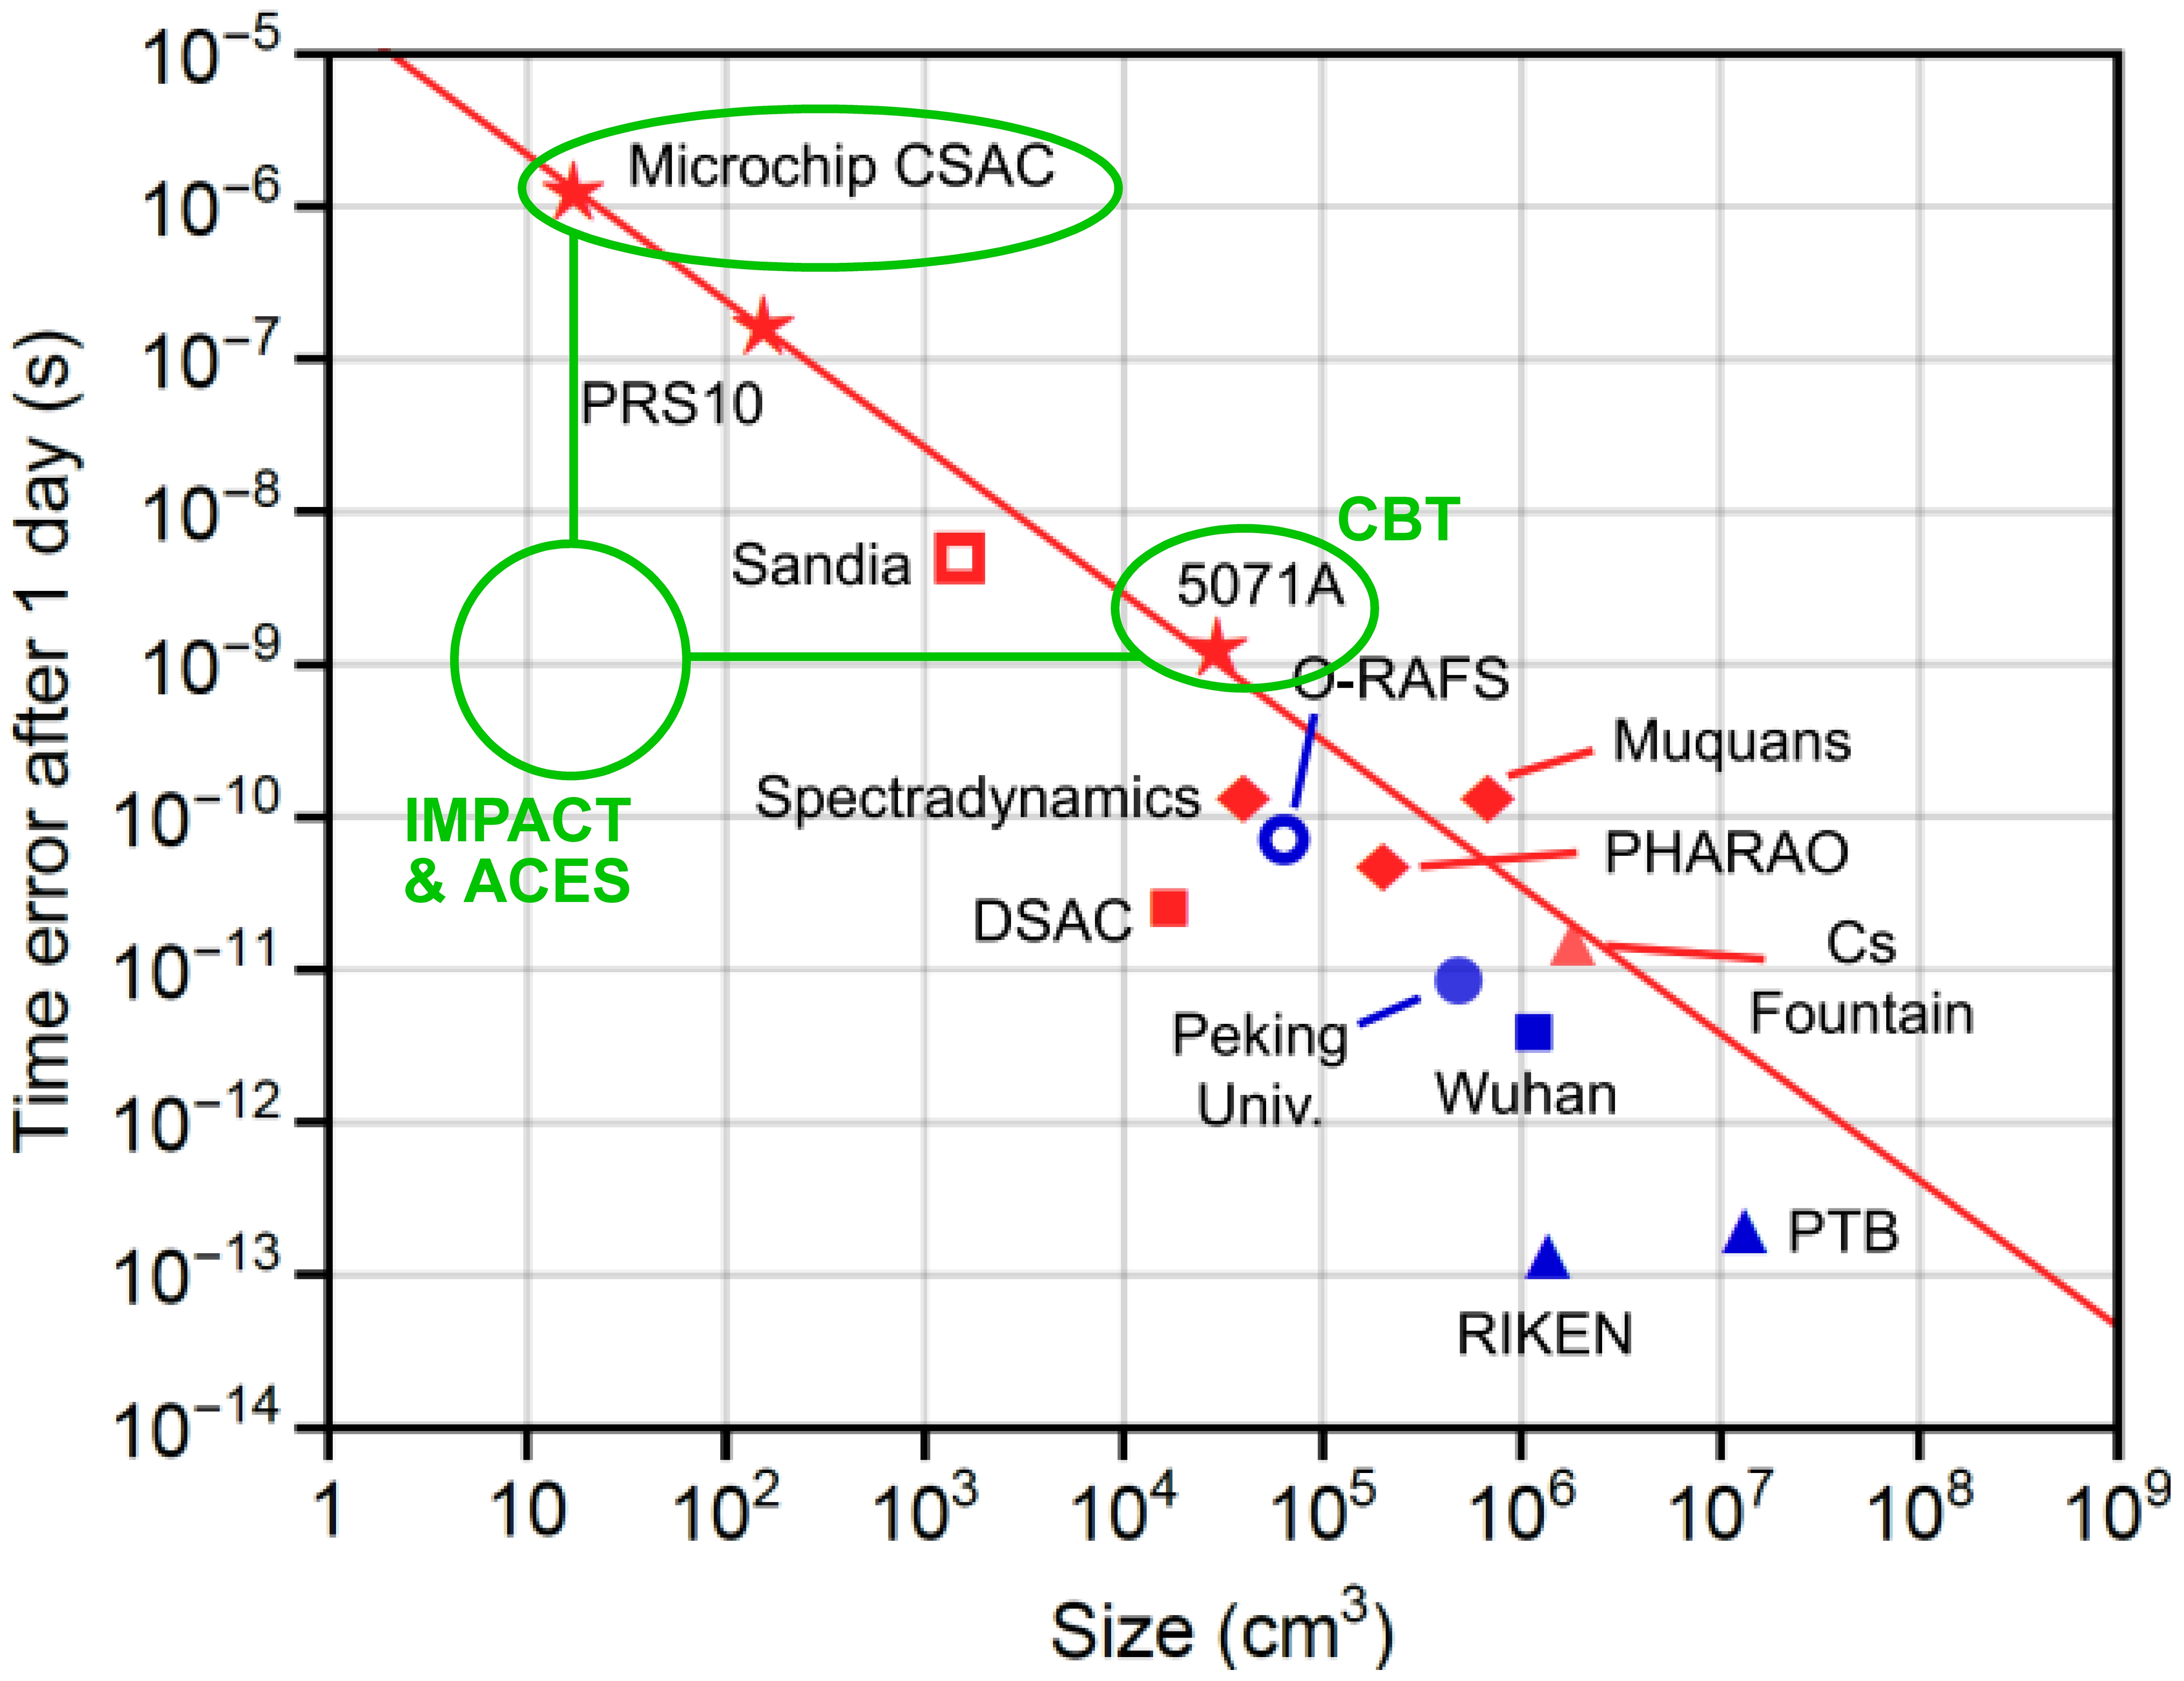
\includegraphics[width=0.6\textwidth, max width=\linewidth]{img/DARPA-stability-target.jpg}
    \caption{Stability targets for the DARPA IMPACT and ACES programs. Source \cite{Marlow-Scherer}.}
    \label{fig:DARPA-stability-target}
\end{figure}

Generally speaking, the next generation of \acrshort{csacs} aims to achieve similar quality in terms pf performances to the current Cesium Beam Tube (CBT) clocks, which are the current gold standard for high-precision timekeeping, while maintaining the advantages of the \acrshort{csac} technology in terms of size, weight and power consumption.


\subsection{Proposed research directions}
\label{subsec:proposed_research_directions}

To overcome the current limitations and deviate from the relation between stability and SWaP explained in Section \ref{subsec:stability_vs_SWaP}, a different physics approach must be exploited.

After more than 15 years since the beginning of the IMPACT program, three main research directions have been identified as the most promising for the development of \acrshort{ngcsacs}:

\begin{itemize}
    \item Microwave transitions in laser-cooled alkali metals.
    \item Microwave transitions in double-resonance trapped ions.
    \item Optical transitions in warm atomic/molecular vapors.
\end{itemize}

In the following subsections, we will analyze the current state of the art of these research directions and the challenges that need to be addressed to make them suitable for commercial applications.


\subsubsection{Microwave transitions in laser-cooled alkali metals}
\label{subsubsec:laser_cooled_alkali}

The first research direction is based on the use of microwave transitions in laser-cooled alkali metals.

The use of cold atoms in the reference cell instead of warm atoms allows for a significant reduction in the Doppler broadening of the atomic transitions and the collisional shifts, which can be considered the main sources of frequency instability in the current \acrshort{csac} technology.

In the proposed architecture, both \acrshort{rb} and \acrshort{cs} atoms are laser-cooled and trapped in a 2D-MOT\footnote{2D Magneto-Optical Trap}, before being transferred to a dedicated interrogation cell.
Here two distinct CPT light fields are used at first to prepare the atoms in a coherent superposition of states, and then to probe the atomic transitions based on the local oscillator frequency.

From a stability point of view, the results look promising as the Doppler broadening is significantly reduced and the line quality factor is greatly improved, allowing for $\sigma_y(\tau=1s) \approx 10^{-11}$ and $\sigma_y(\tau=10^4s) \approx 3 \times 10^{-13}$.
The main bottlenecks are given by the technological and experimental limitations.
In particular, pressure drifts of the atom source, imperfections in the CPT optical implementation, and technical noise on the lasers are the main sources of instability, rather than fundamental physics.


\subsubsection{Microwave transitions in double-resonance trapped ions}
\label{subsubsec:double_resonance_ions}

The second research direction is based on microwave transitions with double-resonance trapped ions.
As of today, this seems to be the most promising path as it allows for a significant reduction in the Doppler broadening while permitting miniaturization of the components.

The working principle is very similar to the one of the laser-cooled alkali metals, but with the use of ions instead of atoms and a different cooling mechanism.
In particular, both Ytterbium ($^{171}Yb^+$) and Mercury ($^{199}Hg^+$) based clocks have been developed and tested, showing excellent stability thanks to the use of Paul's trap mechanism.

A couple of fully functional prototypes have been developed, such as the $^{171}Yb^+$ clock developed by Sandia National Laboratories and NASA's Jet Propulsion Laboratory (JPL) in 2015, and the $^{199}Hg^+$ clock developed by JPL in 2019.

Both the clocks already met the stability requirements imposed by the DARPA programs, but still face some challenges related in particular to Stark effect.
The use of electric fields for ion manipulation can cause a shift in the ions' transition frequency.
To mitigate this, pulsed laser interrogation techniques are required, which indeed complicate the system design and the miniaturization of the components.

On the other hand, the simplicity of the trapping system and the high manipulability of the ions make this approach the most promising in the optics of \acrshort{ngcsacs}.


\subsubsection{Optical transitions in warm atomic/molecular vapors}
\label{subsubsec:optical_transitions}

The third research direction is based on the use of optical transitions in warm atoms environments.

The switching from a microwave range in the target transition frequency to a much higher energy (optical) range allow an increase in both the line quality factor and the signal-to-noise ratio, allowing for a significant improvement in the clock stability ($\sigma_y(\tau=1s) \approx 2 \times 10^{-12}$ and $\sigma_y(\tau=10^3s) \approx 10^{-13}$).

However, this approach is the most challenging from a technological point of view as it requires the fabrication of a series of miniaturized components, such as Kerr-micro-resonator frequency combs, waveguides, and microfabricated photomultiplier tubes.
Those components are still immature from a technological point of view and require further development to be suitable for commercial applications.

At the moment, some earlier version prototypes have been developed, such as the NIST Chip-Scale Optical Atomic Clock in 2019 and the NIST-DRAPER Miniature Atomic Clock in 2020.
As in the case of the other proposed research directions, also these clocks met the stability requirements imposed by the DARPA programs.
The main challenges remain in the miniaturization of the components and their fabrication process at large scale.




% \section{Conclusion}
\label{sec:conclusion}

\acrfull{csacs} represent a significant advancement in the field of atomic clocks, offering a miniaturized and low-power alternative to traditional atomic clocks.
Their enhanced stability and accuracy thanks to the use of atomic transitions as a discipline reference for the local oscillator make them ideal for a wide range of applications, where precise timekeeping and size, weight, and power constraints are critical.

However, the physics enabling the operation of \acrshort{csacs} also poses significant challenges in a further step towards better performance and miniaturization.
Due to the intrinsic limitations, also the applications involving \acrshort{csacs} often relies of some external reference to correct the drift and the aging on the long term.

To overcome these limitations, the development of the next generation of \acrshort{csacs} is an active area of research.
After more than 15 years since the launch of the first program to develop the NG-CSACs, several technological solutions have been proposed, but a clear winner has yet to emerge.

The potential of NG-CSACs is vast, extending far beyond precise timekeeping.
In case of success, these devices have the potential to revolutionize fields like microfabrication, quantum computing, and even our understanding of fundamental physics phenomena.
We believe that pursuing the development goals set for NG-CSACs represents an investment in the future, paving the way for groundbreaking advancements across various scientific and technological disciplines.

% \section*{Acknowledgments}

% \printbibliography

\end{document}
